% Options for packages loaded elsewhere
\PassOptionsToPackage{unicode=true}{hyperref}
\PassOptionsToPackage{hyphens}{url}
%
\documentclass[
]{book}
\usepackage{lmodern}
\usepackage{amssymb,amsmath}
\usepackage{ifxetex,ifluatex}
\ifnum 0\ifxetex 1\fi\ifluatex 1\fi=0 % if pdftex
  \usepackage[T1]{fontenc}
  \usepackage[utf8]{inputenc}
  \usepackage{textcomp} % provides euro and other symbols
\else % if luatex or xelatex
  \usepackage{unicode-math}
  \defaultfontfeatures{Scale=MatchLowercase}
  \defaultfontfeatures[\rmfamily]{Ligatures=TeX,Scale=1}
\fi
% Use upquote if available, for straight quotes in verbatim environments
\IfFileExists{upquote.sty}{\usepackage{upquote}}{}
\IfFileExists{microtype.sty}{% use microtype if available
  \usepackage[]{microtype}
  \UseMicrotypeSet[protrusion]{basicmath} % disable protrusion for tt fonts
}{}
\makeatletter
\@ifundefined{KOMAClassName}{% if non-KOMA class
  \IfFileExists{parskip.sty}{%
    \usepackage{parskip}
  }{% else
    \setlength{\parindent}{0pt}
    \setlength{\parskip}{6pt plus 2pt minus 1pt}}
}{% if KOMA class
  \KOMAoptions{parskip=half}}
\makeatother
\usepackage{xcolor}
\IfFileExists{xurl.sty}{\usepackage{xurl}}{} % add URL line breaks if available
\IfFileExists{bookmark.sty}{\usepackage{bookmark}}{\usepackage{hyperref}}
\hypersetup{
  pdftitle={Evaluating Discards using Observer Data Guyana`s Shrimp Fishery},
  pdfauthor={Seion Richardson},
  hidelinks,
}
\urlstyle{same} % disable monospaced font for URLs
\usepackage{color}
\usepackage{fancyvrb}
\newcommand{\VerbBar}{|}
\newcommand{\VERB}{\Verb[commandchars=\\\{\}]}
\DefineVerbatimEnvironment{Highlighting}{Verbatim}{commandchars=\\\{\}}
% Add ',fontsize=\small' for more characters per line
\usepackage{framed}
\definecolor{shadecolor}{RGB}{248,248,248}
\newenvironment{Shaded}{\begin{snugshade}}{\end{snugshade}}
\newcommand{\AlertTok}[1]{\textcolor[rgb]{0.94,0.16,0.16}{#1}}
\newcommand{\AnnotationTok}[1]{\textcolor[rgb]{0.56,0.35,0.01}{\textbf{\textit{#1}}}}
\newcommand{\AttributeTok}[1]{\textcolor[rgb]{0.77,0.63,0.00}{#1}}
\newcommand{\BaseNTok}[1]{\textcolor[rgb]{0.00,0.00,0.81}{#1}}
\newcommand{\BuiltInTok}[1]{#1}
\newcommand{\CharTok}[1]{\textcolor[rgb]{0.31,0.60,0.02}{#1}}
\newcommand{\CommentTok}[1]{\textcolor[rgb]{0.56,0.35,0.01}{\textit{#1}}}
\newcommand{\CommentVarTok}[1]{\textcolor[rgb]{0.56,0.35,0.01}{\textbf{\textit{#1}}}}
\newcommand{\ConstantTok}[1]{\textcolor[rgb]{0.00,0.00,0.00}{#1}}
\newcommand{\ControlFlowTok}[1]{\textcolor[rgb]{0.13,0.29,0.53}{\textbf{#1}}}
\newcommand{\DataTypeTok}[1]{\textcolor[rgb]{0.13,0.29,0.53}{#1}}
\newcommand{\DecValTok}[1]{\textcolor[rgb]{0.00,0.00,0.81}{#1}}
\newcommand{\DocumentationTok}[1]{\textcolor[rgb]{0.56,0.35,0.01}{\textbf{\textit{#1}}}}
\newcommand{\ErrorTok}[1]{\textcolor[rgb]{0.64,0.00,0.00}{\textbf{#1}}}
\newcommand{\ExtensionTok}[1]{#1}
\newcommand{\FloatTok}[1]{\textcolor[rgb]{0.00,0.00,0.81}{#1}}
\newcommand{\FunctionTok}[1]{\textcolor[rgb]{0.00,0.00,0.00}{#1}}
\newcommand{\ImportTok}[1]{#1}
\newcommand{\InformationTok}[1]{\textcolor[rgb]{0.56,0.35,0.01}{\textbf{\textit{#1}}}}
\newcommand{\KeywordTok}[1]{\textcolor[rgb]{0.13,0.29,0.53}{\textbf{#1}}}
\newcommand{\NormalTok}[1]{#1}
\newcommand{\OperatorTok}[1]{\textcolor[rgb]{0.81,0.36,0.00}{\textbf{#1}}}
\newcommand{\OtherTok}[1]{\textcolor[rgb]{0.56,0.35,0.01}{#1}}
\newcommand{\PreprocessorTok}[1]{\textcolor[rgb]{0.56,0.35,0.01}{\textit{#1}}}
\newcommand{\RegionMarkerTok}[1]{#1}
\newcommand{\SpecialCharTok}[1]{\textcolor[rgb]{0.00,0.00,0.00}{#1}}
\newcommand{\SpecialStringTok}[1]{\textcolor[rgb]{0.31,0.60,0.02}{#1}}
\newcommand{\StringTok}[1]{\textcolor[rgb]{0.31,0.60,0.02}{#1}}
\newcommand{\VariableTok}[1]{\textcolor[rgb]{0.00,0.00,0.00}{#1}}
\newcommand{\VerbatimStringTok}[1]{\textcolor[rgb]{0.31,0.60,0.02}{#1}}
\newcommand{\WarningTok}[1]{\textcolor[rgb]{0.56,0.35,0.01}{\textbf{\textit{#1}}}}
\usepackage{longtable,booktabs}
% Allow footnotes in longtable head/foot
\IfFileExists{footnotehyper.sty}{\usepackage{footnotehyper}}{\usepackage{footnote}}
\makesavenoteenv{longtable}
\usepackage{graphicx,grffile}
\makeatletter
\def\maxwidth{\ifdim\Gin@nat@width>\linewidth\linewidth\else\Gin@nat@width\fi}
\def\maxheight{\ifdim\Gin@nat@height>\textheight\textheight\else\Gin@nat@height\fi}
\makeatother
% Scale images if necessary, so that they will not overflow the page
% margins by default, and it is still possible to overwrite the defaults
% using explicit options in \includegraphics[width, height, ...]{}
\setkeys{Gin}{width=\maxwidth,height=\maxheight,keepaspectratio}
\setlength{\emergencystretch}{3em} % prevent overfull lines
\providecommand{\tightlist}{%
  \setlength{\itemsep}{0pt}\setlength{\parskip}{0pt}}
\setcounter{secnumdepth}{5}
% Redefines (sub)paragraphs to behave more like sections
\ifx\paragraph\undefined\else
  \let\oldparagraph\paragraph
  \renewcommand{\paragraph}[1]{\oldparagraph{#1}\mbox{}}
\fi
\ifx\subparagraph\undefined\else
  \let\oldsubparagraph\subparagraph
  \renewcommand{\subparagraph}[1]{\oldsubparagraph{#1}\mbox{}}
\fi

% Set default figure placement to htbp
\makeatletter
\def\fps@figure{htbp}
\makeatother

\usepackage{booktabs}
\usepackage{amsthm}
\makeatletter
\def\thm@space@setup{%
  \thm@preskip=8pt plus 2pt minus 4pt
  \thm@postskip=\thm@preskip
}
\makeatother
\usepackage{booktabs}
\usepackage{longtable}
\usepackage{array}
\usepackage{multirow}
\usepackage{wrapfig}
\usepackage{float}
\usepackage{colortbl}
\usepackage{pdflscape}
\usepackage{tabu}
\usepackage{threeparttable}
\usepackage{threeparttablex}
\usepackage[normalem]{ulem}
\usepackage{makecell}
\usepackage{xcolor}
\usepackage[]{natbib}
\bibliographystyle{apalike}

\title{Evaluating Discards using Observer Data Guyana`s Shrimp Fishery}
\author{Seion Richardson}
\date{2020-11-12}

\begin{document}
\maketitle

{
\setcounter{tocdepth}{1}
\tableofcontents
}
\hypertarget{chapter}{%
\chapter{CHAPTER}\label{chapter}}

\hypertarget{key-definitions}{%
\section{Key definitions}\label{key-definitions}}

\textbf{Total catch} - the amount of fish caught by a fishing gear that reaches the vessels deck.
\textbf{Target catch} - the main species which are sought after by a particular fishery e.g.~cod or shrimp.
\textbf{Incidental catch} - the species caught which are retained for consumption or marketing purposes.
\textbf{Discarded catch} - the section of catch returned to the sea, usually dead or alive.
\textbf{Bycatch} - Discarded catch combined with incidental catch.
\textbf{Fishery observer} - is a specialist trained in collecting data onboard commercial fishing vessels.
\textbf{Observer data} - data collected at-sea by fishery observers.
\textbf{Tow} - The act of fishing or trawling.
\textbf{CPUE} - Catch per unit effort i.e.~the fish caught per unit of fishing effort e.g.~kgs/hr.

\hypertarget{introduction}{%
\section{Introduction}\label{introduction}}

The data used in this project is on discarded fish species (Appendix 4.1) from the Atlantic seabob(Appendix 4.3) fishery in Guyana, South America (Figure 1). The data was collected at-sea by fishery observers (Figure 2) onboard seven Atlantic seabob shrimp bottom trawl vessels (Appendix 4.2) between 2019 to 2020 (see chapter 1.3 for data variables). The data was collected within the seabob trawling zone i.e.~15 to 33 metres of water depth (Figure 1). It includes sampled bottom trawl fishing tow data from eight distinct fishing trips (one vessel was used twice) with an average of six sampled hauls per trip (three day, three night) and at different fishing depths (shallow, deep). Time of day are split into day (6:00HRS to 17:59HRS) and night (18:00HRS to 5:59HRS). Fishing depths are split into deep (\textgreater{} 16.46 metres) and shallow (\textless= 16.46 metres) of water depths. Based on interactions with fisherfolks in Guyana, discarding of fish species from Guyana`s main shrimp fishery is said to be excessive. Therefore this issue will be closely examined in this project, with specific emphasis on species weights and lengths; across varying time of day and fishing depths.

All functions and function arguments in this project are followed directly by parenthesis i.e.~(). So for example: filter() means \textbf{filter() function} and sum() means \textbf{sum() function}. Therefore the word ``function'' will not be used but is implied. To not be repetitive and to make the codes more readable: code comments will only be made the first time that the code is used. Code comments are placed after each object produced from a code chunk. Two examples of these objects are tables or figures.

\hypertarget{fishing-area}{%
\subsection{Fishing Area}\label{fishing-area}}

\begin{figure}
\centering
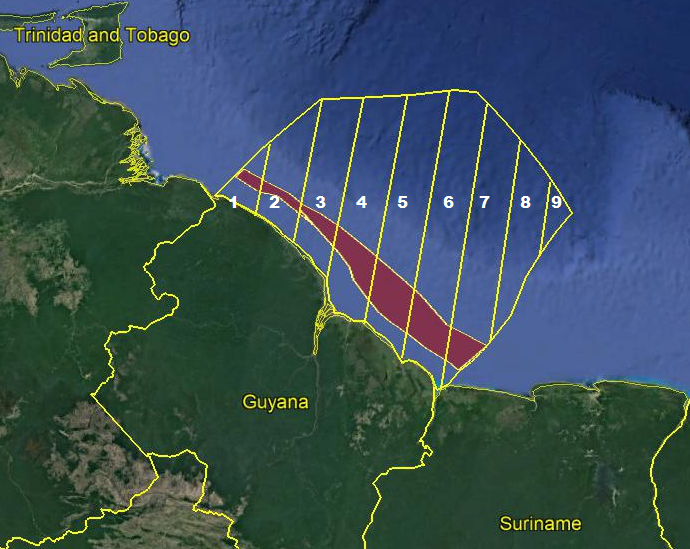
\includegraphics[width=0.65\textwidth,height=\textheight]{C:/Users/UNUFTP/Documents/mas102m/GuyanaEEZ.png}
\caption{Figure 1 Map of Guyana`s 200 nautical miles Exclusive Economic Zone (EEZ). The Yellow boundary lines represents the different maritime boundary zones. The Atlantic seabob fishing zone (i.e.~15 to 33 meter lines) is represented by the area shaded in red (Richardson, 2020).}
\end{figure}

\hypertarget{sampling-protocol-used-to-collect-data}{%
\subsection{Sampling protocol used to collect data}\label{sampling-protocol-used-to-collect-data}}

\begin{figure}
\centering
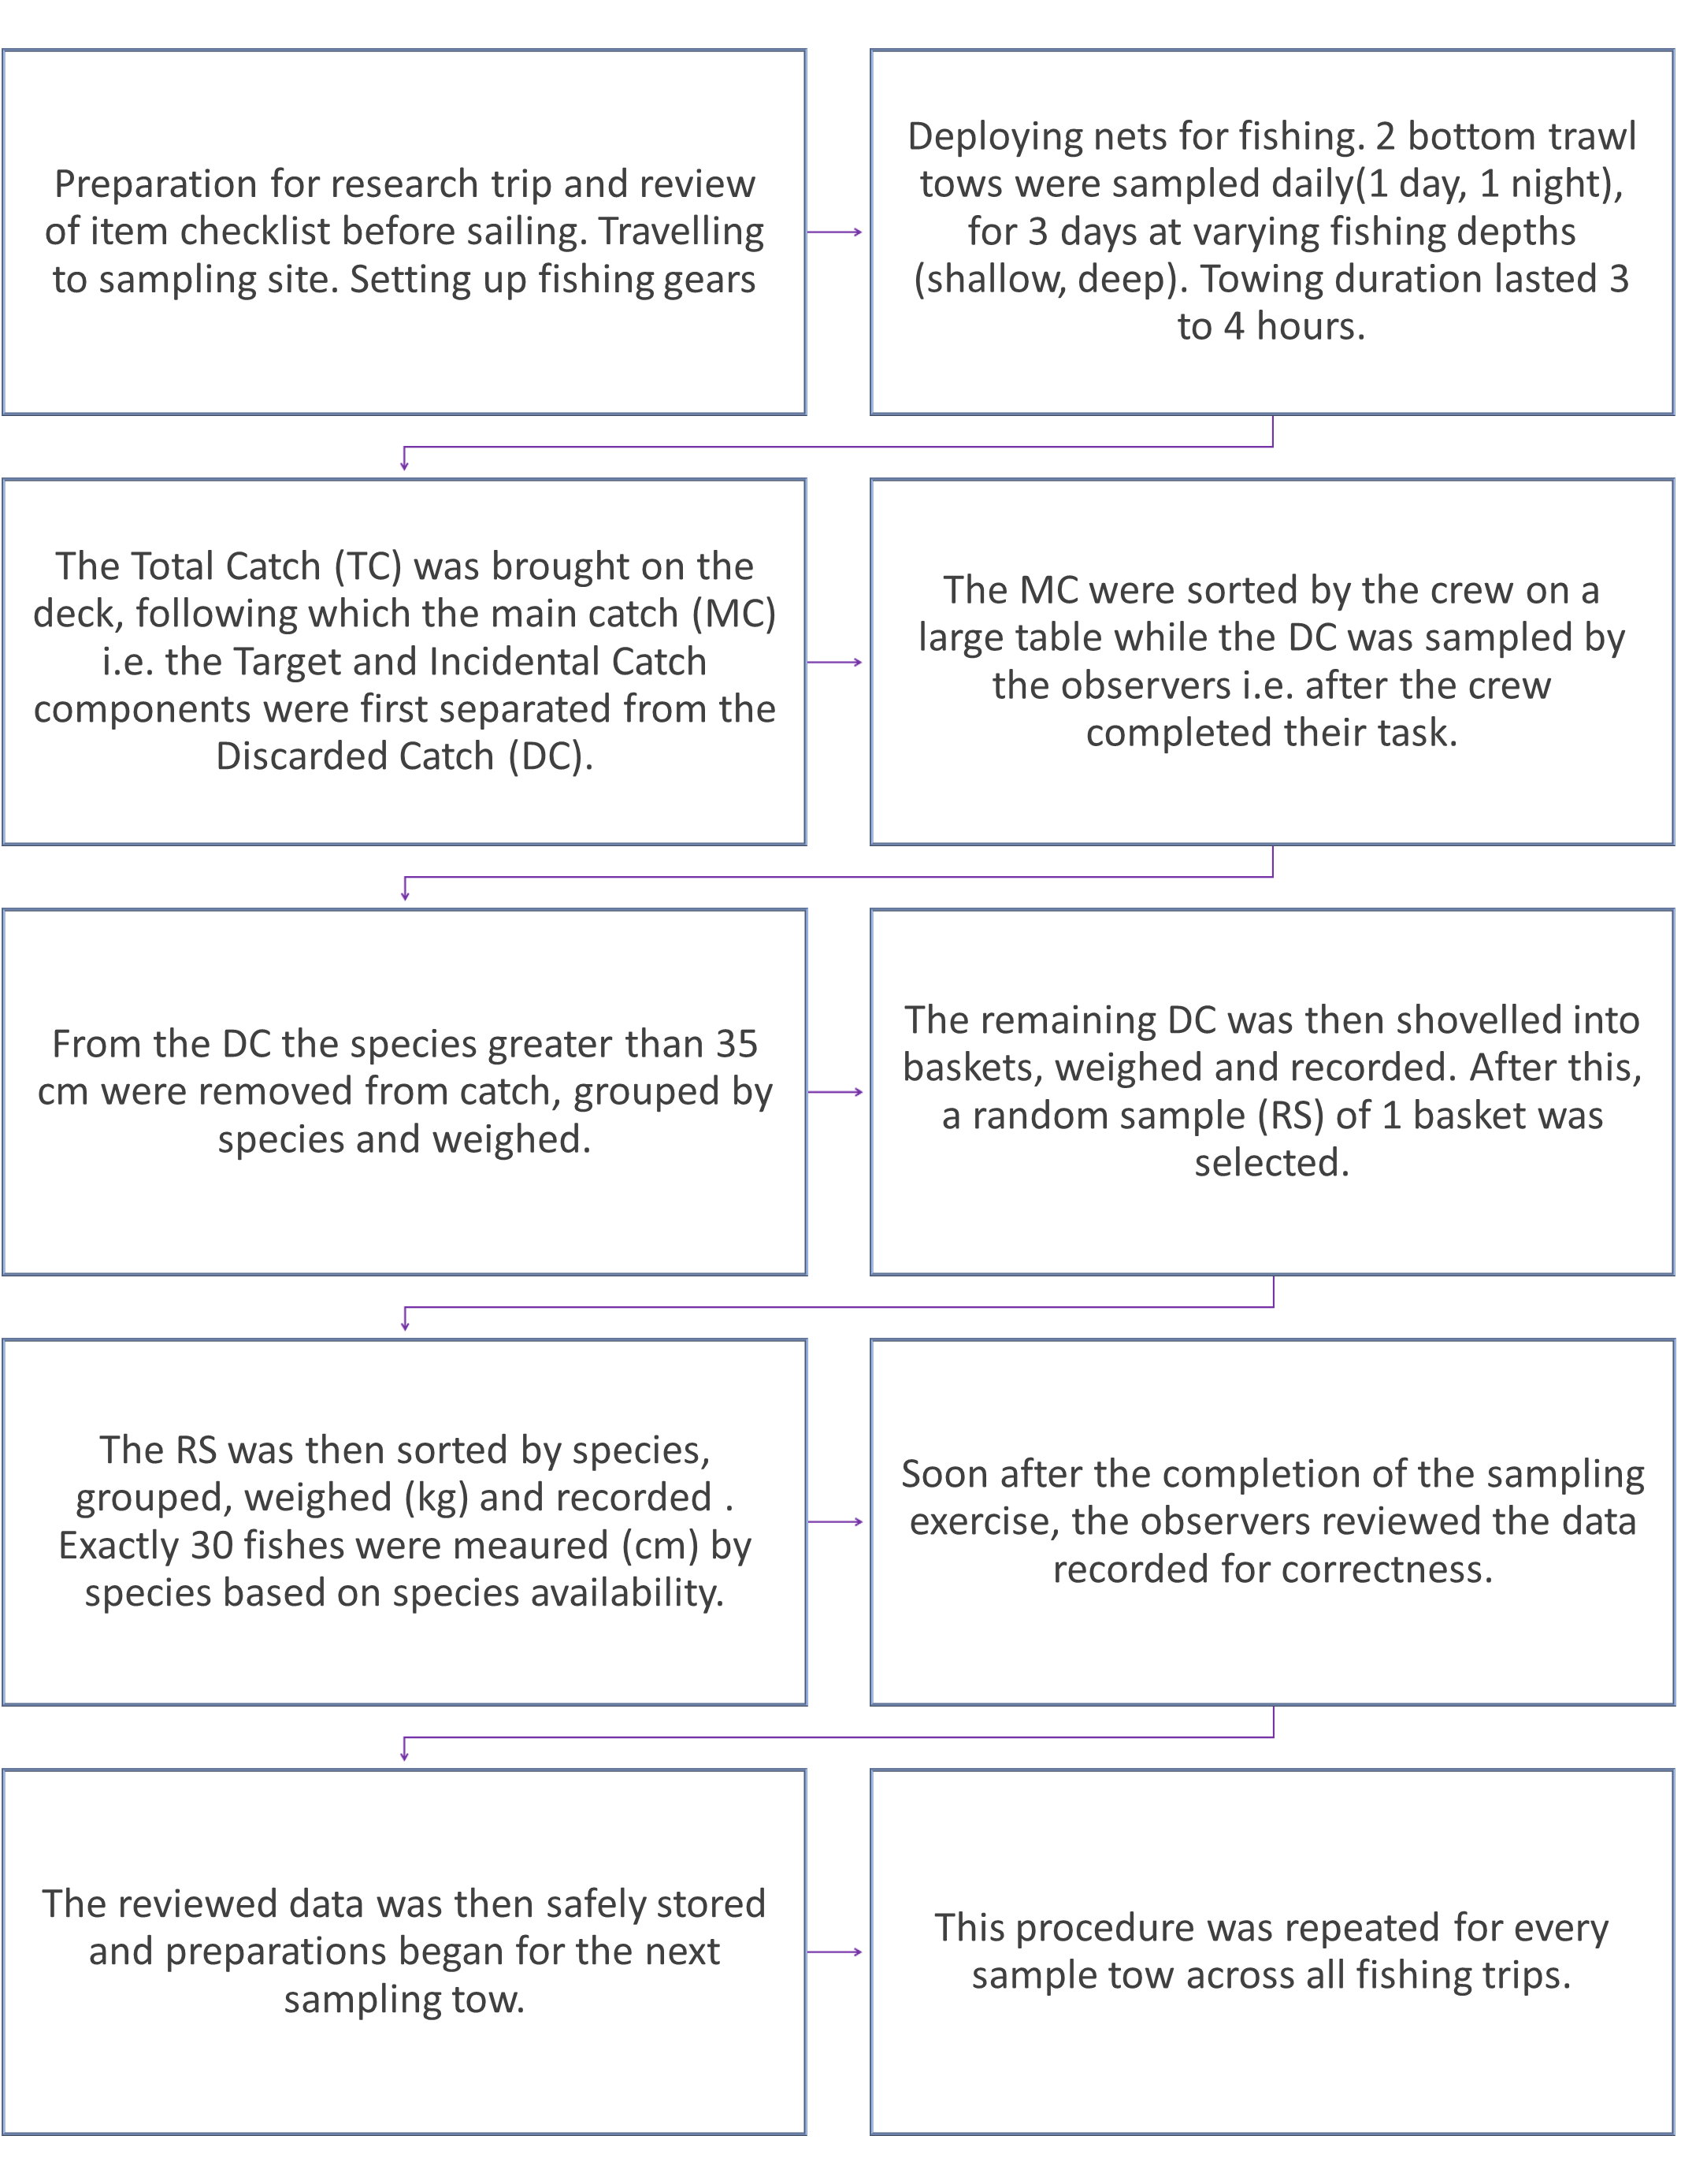
\includegraphics[width=0.75\textwidth,height=\textheight]{C:/Users/UNUFTP/Documents/mas102m/SamplingProtocol2.png}
\caption{Figure 2 Data collection sampling protocol used to collect the data for this project}
\end{figure}

\hypertarget{data-manipulation}{%
\section{Data manipulation}\label{data-manipulation}}

\textbf{R packages used in this project}

\begin{Shaded}
\begin{Highlighting}[]
\KeywordTok{library}\NormalTok{(tidyverse) }\CommentTok{#[1]. Summarize data and make plots}
\KeywordTok{library}\NormalTok{(skimr) }\CommentTok{#[2]. Summarizes data with descriptive statistics}
\KeywordTok{library}\NormalTok{(flextable) }\CommentTok{#[3]. Creates neat tables }
\KeywordTok{library}\NormalTok{(kableExtra) }\CommentTok{#[4]. Also creates tables }
\KeywordTok{library}\NormalTok{(bookdown) }\CommentTok{#[5]. Use to build this html book}
\end{Highlighting}
\end{Shaded}

\textbf{Importing data}

\begin{Shaded}
\begin{Highlighting}[]
\CommentTok{# Reading in csv file with data}
\NormalTok{ObserverData <-}\StringTok{ }\KeywordTok{read_csv}\NormalTok{(}\StringTok{"observer_weights_mas102m.csv"}\NormalTok{)}

\KeywordTok{names}\NormalTok{(ObserverData)}
\end{Highlighting}
\end{Shaded}

\begin{verbatim}
   [1] "company"         "dep_date"        "arr_date"        "das"            
   [5] "trip"            "drag"            "drag_all"        "drag_date"      
   [9] "day"             "month"           "year"            "zone"           
  [13] "drag_period"     "drag_time_s"     "drag_time_e"     "time_fished_min"
  [17] "hrs_dec"         "depth"           "depth_sd"        "id_status"      
  [21] "com_status"      "order"           "family"          "class"          
  [25] "total_catch_cat" "total_catch_spp" "categories"      "sci_name"       
  [29] "alpha_code"      "com_name"        "sample_wt_lbs"   "total_wt_lbs"
\end{verbatim}

\begin{Shaded}
\begin{Highlighting}[]
\KeywordTok{dim}\NormalTok{(ObserverData)}
\end{Highlighting}
\end{Shaded}

\begin{verbatim}
  [1] 1217   32
\end{verbatim}

\begin{Shaded}
\begin{Highlighting}[]
\CommentTok{### CODE COMMENTS }\AlertTok{###}
\CommentTok{#[1]. Importing the observer data using read_csv() from the tidyverse package.}
\CommentTok{#     The imported data is called "ObserverData" in this project.}
\CommentTok{#[2]. names() from base R is used to print the names of the variables in the data. }
\CommentTok{#[3]. dim() is used to show the length (1217 rows) and width (32 columns) of the imported data. }
\end{Highlighting}
\end{Shaded}

\textbf{Inspecting the classes of variables}

\begin{Shaded}
\begin{Highlighting}[]
\NormalTok{ObserverData }\OperatorTok\StringTok{ }
\StringTok{  }\KeywordTok{glimpse}\NormalTok{()}
\end{Highlighting}
\end{Shaded}

\begin{verbatim}
  Rows: 1,217
  Columns: 32
  $ company         <chr> "NHS", "NHS", "NHS", "NHS", "NHS", "NHS", "NHS", "N...
  $ dep_date        <chr> "14/02/2019", "14/02/2019", "14/02/2019", "14/02/20...
  $ arr_date        <chr> "24/02/2019", "24/02/2019", "24/02/2019", "24/02/20...
  $ das             <dbl> 11, 11, 11, 11, 11, 11, 11, 11, 11, 11, 11, 11, 11,...
  $ trip            <dbl> 1, 1, 1, 1, 1, 1, 1, 1, 1, 1, 1, 1, 1, 1, 1, 1, 1, ...
  $ drag            <dbl> 1, 1, 1, 1, 1, 1, 1, 1, 1, 1, 1, 1, 1, 1, 1, 1, 1, ...
  $ drag_all        <dbl> 1, 1, 1, 1, 1, 1, 1, 1, 1, 1, 1, 1, 1, 1, 1, 1, 1, ...
  $ drag_date       <chr> "15/02/2019", "15/02/2019", "15/02/2019", "15/02/20...
  $ day             <dbl> 15, 15, 15, 15, 15, 15, 15, 15, 15, 15, 15, 15, 15,...
  $ month           <dbl> 2, 2, 2, 2, 2, 2, 2, 2, 2, 2, 2, 2, 2, 2, 2, 2, 2, ...
  $ year            <dbl> 2019, 2019, 2019, 2019, 2019, 2019, 2019, 2019, 201...
  $ zone            <dbl> 6, 6, 6, 6, 6, 6, 6, 6, 6, 6, 6, 6, 6, 6, 6, 6, 6, ...
  $ drag_period     <chr> "Day", "Day", "Day", "Day", "Day", "Day", "Day", "D...
  $ drag_time_s     <time> 08:00:00, 08:00:00, 08:00:00, 08:00:00, 08:00:00, ...
  $ drag_time_e     <time> 12:00:00, 12:00:00, 12:00:00, 12:00:00, 12:00:00, ...
  $ time_fished_min <time> 04:00:00, 04:00:00, 04:00:00, 04:00:00, 04:00:00, ...
  $ hrs_dec         <dbl> 4, 4, 4, 4, 4, 4, 4, 4, 4, 4, 4, 4, 4, 4, 4, 4, 4, ...
  $ depth           <dbl> 10, 10, 10, 10, 10, 10, 10, 10, 10, 10, 10, 10, 10,...
  $ depth_sd        <chr> "Deep", "Deep", "Deep", "Deep", "Deep", "Deep", "De...
  $ id_status       <chr> "Yes", "Yes", "Yes", "Yes", "Yes", "Yes", "Yes", "Y...
  $ com_status      <chr> "No", "Yes", "No", "Yes", "Yes", "Yes", "No", "No",...
  $ order           <chr> "Perciformes", "Perciformes", "Decapoda", "Percifor...
  $ family          <chr> "Sciaenidae", "Sciaenidae", "Malacostraca", "Sciaen...
  $ class           <chr> "Actinopterygii", "Actinopterygii", "Malacostraca",...
  $ total_catch_cat <chr> "Discarded catch", "Discarded catch", "Discarded ca...
  $ total_catch_spp <chr> "Bycatch species", "Bycatch species", "Bycatch spec...
  $ categories      <chr> "Bony fish", "Bony fish", "Shell fish", "Bony fish"...
  $ sci_name        <chr> "Paralonchurus brasiliensis", "Macrodon ancylodon",...
  $ alpha_code      <chr> "RLB", "WKK", "HGV", "NBM", "BEB", "RLE", "EFM", "E...
  $ com_name        <chr> "Banded croaker", "Bangamary", "Box crab", "Butterf...
  $ sample_wt_lbs   <dbl> 0.50, 3.00, 0.70, 3.00, 4.30, 6.30, 12.00, 20.00, 0...
  $ total_wt_lbs    <dbl> 1.26, 7.58, 1.77, 7.58, 10.87, 15.93, 30.34, 50.57,...
\end{verbatim}

\begin{Shaded}
\begin{Highlighting}[]
\CommentTok{### CODE COMMENTS }\AlertTok{###}
\CommentTok{#[1]. glimpse() is used to view the classes of each variable from the data. }
\end{Highlighting}
\end{Shaded}

From the output created above we can see that of the 32 variables, 17 were of class characters, 3 difftime and 12 numeric. All the data seems to fit reasonably well into the required categories i.e.~character, difftime and numeric. The main exceptions were the dates variables. Normally, these would have needed to be converted before use. However, this will not be done in this project as dates are not required to answer the research questions.

\textbf{Description of data variables}

The variables within the data are coded. A total of 32 variables were recorded in the data. A description for each variable is below :

\begin{enumerate}
\def\labelenumi{\arabic{enumi}.}
\tightlist
\item
  \textbf{company}: Fishing company
\item
  \textbf{dep\_date}: Date the vessel departs port for fishing
\item
  \textbf{arr\_date}: Date the vessel returns from fishing
\item
  \textbf{das}: Number of days the vessel spent at-sea\\
\item
  \textbf{trip}: Unique trip identification number
\item
  \textbf{drag}: Unique drag identification number by
\item
  \textbf{drag\_all}: Sequential drag identification number
\item
  \textbf{drag\_date}: Date the drag was done
\item
  \textbf{day}: Day the drag was done
\item
  \textbf{month}: Month the drag was done
\item
  \textbf{year}: Year the drag was done
\item
  \textbf{zone}: Fishing zone (Figure 1) where the drag was done
\item
  \textbf{drag\_period}: Binary variable of time of day for drag
\item
  \textbf{drag\_time\_s}: Time the drag started (24:00 hrs)
\item
  \textbf{drag\_time\_e}: Time the drag ended (24:00 hrs)
\item
  \textbf{time\_fished\_min}: Time fished in hours
\item
  \textbf{hrs\_dec}: Time fished converted to decimals
\item
  \textbf{depth}: Average fishing depth
\item
  \textbf{depth\_sd}: Binary variable of fishing depth
\item
  \textbf{id\_status}: Binary variable of species identification
\item
  \textbf{com\_status}: Binary variable of species economic status
\item
  \textbf{order}: Species taxonomy - Order
\item
  \textbf{family}: Species taxonomy - Family
\item
  \textbf{class}: Species taxonomy - Class
\item
  \textbf{total\_catch\_cat}: Catch categorization (see definitions)
\item
  \textbf{total\_catch\_spp}: Board species categorization
\item
  \textbf{categories}: More narrow species categorization 
\item
  \textbf{sci\_name}: Latin names for each species
\item
  \textbf{alpha\_code}: Unique 3-alpha species identifier used by FAO
\item
  \textbf{com\_name}: Local name or ``call name'' for species
\item
  \textbf{sample\_wt\_lbs}: Species sample weight per drag (in lbs)
\item
  \textbf{total\_wt\_lbs}: Species total weight per drag (in lbs)
\end{enumerate}

\emph{However, most of them will not be required in this project.}

\textbf{Printing the first 6 rows of the data}

\begin{Shaded}
\begin{Highlighting}[]
\NormalTok{HeadData <-}\StringTok{ }\KeywordTok{head}\NormalTok{(ObserverData) }

\NormalTok{HeadData }\OperatorTok\StringTok{ }
\StringTok{  }\KeywordTok{kbl}\NormalTok{(}\DataTypeTok{caption =} \StringTok{"The first six rows of data"}\NormalTok{) }\OperatorTok
\StringTok{  }\KeywordTok{kable_classic}\NormalTok{() }\OperatorTok
\StringTok{  }\KeywordTok{row_spec}\NormalTok{(}\DecValTok{0}\NormalTok{, }\DataTypeTok{bold =} \OtherTok{TRUE}\NormalTok{) }\OperatorTok
\StringTok{  }\KeywordTok{kable_styling}\NormalTok{(}\DataTypeTok{fixed_thead =}\NormalTok{ T,}
    \DataTypeTok{bootstrap_options =} \KeywordTok{c}\NormalTok{(}\StringTok{"striped"}\NormalTok{,}
      \StringTok{"condensed"}\NormalTok{)) }\OperatorTok\StringTok{ }
\StringTok{  }\KeywordTok{scroll_box}\NormalTok{(}\DataTypeTok{width =} \StringTok{"770px"}\NormalTok{, }\DataTypeTok{height =} \StringTok{"350px"}\NormalTok{)}
\end{Highlighting}
\end{Shaded}

\begin{table}

\caption{\label{tab:unnamed-chunk-2}The first six rows of data}
\centering
\begin{tabular}[t]{l|l|l|r|r|r|r|l|r|r|r|r|l|l|l|l|r|r|l|l|l|l|l|l|l|l|l|l|l|l|r|r}
\hline
\textbf{company} & \textbf{dep\_date} & \textbf{arr\_date} & \textbf{das} & \textbf{trip} & \textbf{drag} & \textbf{drag\_all} & \textbf{drag\_date} & \textbf{day} & \textbf{month} & \textbf{year} & \textbf{zone} & \textbf{drag\_period} & \textbf{drag\_time\_s} & \textbf{drag\_time\_e} & \textbf{time\_fished\_min} & \textbf{hrs\_dec} & \textbf{depth} & \textbf{depth\_sd} & \textbf{id\_status} & \textbf{com\_status} & \textbf{order} & \textbf{family} & \textbf{class} & \textbf{total\_catch\_cat} & \textbf{total\_catch\_spp} & \textbf{categories} & \textbf{sci\_name} & \textbf{alpha\_code} & \textbf{com\_name} & \textbf{sample\_wt\_lbs} & \textbf{total\_wt\_lbs}\\
\hline
NHS & 14/02/2019 & 24/02/2019 & 11 & 1 & 1 & 1 & 15/02/2019 & 15 & 2 & 2019 & 6 & Day & 08:00:00 & 12:00:00 & 04:00:00 & 4 & 10 & Deep & Yes & No & Perciformes & Sciaenidae & Actinopterygii & Discarded catch & Bycatch species & Bony fish & Paralonchurus brasiliensis & RLB & Banded croaker & 0.5 & 1.26\\
\hline
NHS & 14/02/2019 & 24/02/2019 & 11 & 1 & 1 & 1 & 15/02/2019 & 15 & 2 & 2019 & 6 & Day & 08:00:00 & 12:00:00 & 04:00:00 & 4 & 10 & Deep & Yes & Yes & Perciformes & Sciaenidae & Actinopterygii & Discarded catch & Bycatch species & Bony fish & Macrodon ancylodon & WKK & Bangamary & 3.0 & 7.58\\
\hline
NHS & 14/02/2019 & 24/02/2019 & 11 & 1 & 1 & 1 & 15/02/2019 & 15 & 2 & 2019 & 6 & Day & 08:00:00 & 12:00:00 & 04:00:00 & 4 & 10 & Deep & Yes & No & Decapoda & Malacostraca & Malacostraca & Discarded catch & Bycatch species & Shell fish & Hepatus gronovii & HGV & Box crab & 0.7 & 1.77\\
\hline
NHS & 14/02/2019 & 24/02/2019 & 11 & 1 & 1 & 1 & 15/02/2019 & 15 & 2 & 2019 & 6 & Day & 08:00:00 & 12:00:00 & 04:00:00 & 4 & 10 & Deep & Yes & Yes & Perciformes & Sciaenidae & Actinopterygii & Discarded catch & Bycatch species & Bony fish & Nebris microps & NBM & Butterfish & 3.0 & 7.58\\
\hline
NHS & 14/02/2019 & 24/02/2019 & 11 & 1 & 1 & 1 & 15/02/2019 & 15 & 2 & 2019 & 6 & Day & 08:00:00 & 12:00:00 & 04:00:00 & 4 & 10 & Deep & Yes & Yes & Siluriformes & Ariidae & Actinopterygii & Discarded catch & Bycatch species & Bony fish & Bagre bagre & BEB & Catfish & 4.3 & 10.87\\
\hline
NHS & 14/02/2019 & 24/02/2019 & 11 & 1 & 1 & 1 & 15/02/2019 & 15 & 2 & 2019 & 6 & Day & 08:00:00 & 12:00:00 & 04:00:00 & 4 & 10 & Deep & Yes & Yes & Perciformes & Sciaenidae & Actinopterygii & Discarded catch & Bycatch species & Bony fish & Lonchurus elegans & RLE & Chinese butterfish & 6.3 & 15.93\\
\hline
\end{tabular}
\end{table}

\begin{Shaded}
\begin{Highlighting}[]
\CommentTok{### CODE COMMENTS }\AlertTok{###}
\CommentTok{#[1]. A peek at first 6 rows in data using head().}
\CommentTok{#[2]. kable() is used to create a scrollable html table. This is useful for data with many variables }
\CommentTok{#     like this one. }
\end{Highlighting}
\end{Shaded}

\textbf{Renaming of all the variables from the data}

\begin{Shaded}
\begin{Highlighting}[]
\NormalTok{ObserverData <-}\StringTok{  }\NormalTok{ObserverData }\OperatorTok\StringTok{ }
\StringTok{  }\NormalTok{dplyr}\OperatorTok{::}\KeywordTok{rename}\NormalTok{(}\DataTypeTok{Company =}\NormalTok{ company, }
                \DataTypeTok{Departure =}\NormalTok{ dep_date,}
                \DataTypeTok{Arrival =}\NormalTok{ arr_date, }
                \DataTypeTok{DaysAtSea =}\NormalTok{ das, }
                \DataTypeTok{TripID =}\NormalTok{ trip, }
                \DataTypeTok{DragID =}\NormalTok{ drag, }
                \DataTypeTok{DragID2 =}\NormalTok{ drag_all, }
                \DataTypeTok{DragDate =}\NormalTok{ drag_date,}
                \DataTypeTok{Day =}\NormalTok{ day,}
                \DataTypeTok{Month =}\NormalTok{ month,}
                \DataTypeTok{Year =}\NormalTok{ year,}
                \DataTypeTok{Zone =}\NormalTok{ zone,}
                \DataTypeTok{TimePeriods =}\NormalTok{ drag_period, }
                \DataTypeTok{DragStart =}\NormalTok{ drag_time_s, }
                \DataTypeTok{DragEnd =}\NormalTok{ drag_time_e, }
                \DataTypeTok{TimeFishedHrs =}\NormalTok{ time_fished_min, }
                \DataTypeTok{TimeFishedDec =}\NormalTok{ hrs_dec, }
                \DataTypeTok{FishingDepth =}\NormalTok{ depth, }
                \DataTypeTok{FishingDepth2 =}\NormalTok{ depth_sd, }
                \DataTypeTok{SpeciesID =}\NormalTok{ id_status, }
                \DataTypeTok{EconomicStatus =}\NormalTok{ com_status, }
                \DataTypeTok{OrderTax =}\NormalTok{ order, }
                \DataTypeTok{FamilyTax =}\NormalTok{ family, }
                \DataTypeTok{ClassTax =}\NormalTok{ class, }
                \DataTypeTok{CatchCategory =}\NormalTok{ total_catch_cat, }
                \DataTypeTok{SpeciesCategory =}\NormalTok{ total_catch_spp, }
                \DataTypeTok{SpeciesCategory2 =}\NormalTok{ categories, }
                \DataTypeTok{LatinNames =}\NormalTok{ sci_name, }
                \DataTypeTok{AplhaCode =}\NormalTok{ alpha_code, }
                \DataTypeTok{CommonName =}\NormalTok{ com_name, }
                \DataTypeTok{SampleWeightLB =}\NormalTok{ sample_wt_lbs, }
                \DataTypeTok{TotalWeightLB =}\NormalTok{ total_wt_lbs)}

\KeywordTok{names}\NormalTok{(ObserverData)}
\end{Highlighting}
\end{Shaded}

\begin{verbatim}
   [1] "Company"          "Departure"        "Arrival"          "DaysAtSea"       
   [5] "TripID"           "DragID"           "DragID2"          "DragDate"        
   [9] "Day"              "Month"            "Year"             "Zone"            
  [13] "TimePeriods"      "DragStart"        "DragEnd"          "TimeFishedHrs"   
  [17] "TimeFishedDec"    "FishingDepth"     "FishingDepth2"    "SpeciesID"       
  [21] "EconomicStatus"   "OrderTax"         "FamilyTax"        "ClassTax"        
  [25] "CatchCategory"    "SpeciesCategory"  "SpeciesCategory2" "LatinNames"      
  [29] "AplhaCode"        "CommonName"       "SampleWeightLB"   "TotalWeightLB"
\end{verbatim}

\begin{Shaded}
\begin{Highlighting}[]
\CommentTok{### CODE COMMENTS }\AlertTok{###}
\CommentTok{#[1]. rename() from the dplyr package is used to give the variables descriptive names. }
\CommentTok{#[2]. A quick view of the renamed variables using names() from base R.}
\end{Highlighting}
\end{Shaded}

\textbf{Creating a few additional variables}

Three new variables are being added. These variables will change the current weight units from \textbf{Imperial} to \textbf{Metric} (i.e.~pounds to kilograms) which is more common in Europe.

\begin{Shaded}
\begin{Highlighting}[]
\NormalTok{ObserverData <-}\StringTok{ }\NormalTok{ObserverData }\OperatorTok\StringTok{ }
\StringTok{  }\KeywordTok{mutate}\NormalTok{(}\DataTypeTok{SampleWeightKG =}\NormalTok{ SampleWeightLB}\OperatorTok{/}\FloatTok{2.2}\NormalTok{, }
    \DataTypeTok{TotalWeightKG =}\NormalTok{ TotalWeightLB}\OperatorTok{/}\FloatTok{2.2}\NormalTok{,}
    \DataTypeTok{CpueKGHR =}\NormalTok{ TotalWeightKG}\OperatorTok{/}\NormalTok{TimeFishedDec)}

\KeywordTok{names}\NormalTok{(ObserverData)}
\end{Highlighting}
\end{Shaded}

\begin{verbatim}
   [1] "Company"          "Departure"        "Arrival"          "DaysAtSea"       
   [5] "TripID"           "DragID"           "DragID2"          "DragDate"        
   [9] "Day"              "Month"            "Year"             "Zone"            
  [13] "TimePeriods"      "DragStart"        "DragEnd"          "TimeFishedHrs"   
  [17] "TimeFishedDec"    "FishingDepth"     "FishingDepth2"    "SpeciesID"       
  [21] "EconomicStatus"   "OrderTax"         "FamilyTax"        "ClassTax"        
  [25] "CatchCategory"    "SpeciesCategory"  "SpeciesCategory2" "LatinNames"      
  [29] "AplhaCode"        "CommonName"       "SampleWeightLB"   "TotalWeightLB"   
  [33] "SampleWeightKG"   "TotalWeightKG"    "CpueKGHR"
\end{verbatim}

\begin{Shaded}
\begin{Highlighting}[]
\KeywordTok{dim}\NormalTok{(ObserverData)}
\end{Highlighting}
\end{Shaded}

\begin{verbatim}
  [1] 1217   35
\end{verbatim}

\begin{Shaded}
\begin{Highlighting}[]
\CommentTok{### CODE COMMENTS }\AlertTok{###}
\CommentTok{#[1]. Convert from pounds to kilograms.}
\CommentTok{#[2]. mutate() from the dplyr package is passed to the data "ObserverData" to create three new variables: }
\CommentTok{#     "SampleWeightKG", "TotalweightKG" and "CpueKGHR".}
\CommentTok{#[3]. A quick view of the new variables using names() from base R.}
\end{Highlighting}
\end{Shaded}

The \textbf{ObserverData} data now comprises 35 variables and 1217 row observations.

\hypertarget{inspecting-the-primary-research-variables}{%
\section{Inspecting the primary research variables}\label{inspecting-the-primary-research-variables}}

This research will look into discarded fish species \emph{weights} and \emph{lengths}. These variables will be measured across \emph{time of day} and \emph{fishing depths}.

\hypertarget{count-of-species-sampled-across-fishing-trips-and-time-of-day}{%
\subsection{Count of species sampled across fishing trips and time of day}\label{count-of-species-sampled-across-fishing-trips-and-time-of-day}}

\begin{Shaded}
\begin{Highlighting}[]
\NormalTok{DiscardData <-}\StringTok{ }\NormalTok{ObserverData }\OperatorTok
\StringTok{  }\KeywordTok{filter}\NormalTok{(CatchCategory }\OperatorTok{==}\StringTok{ "Discarded catch"}\NormalTok{)}

\NormalTok{Table.}\FloatTok{1.2}\NormalTok{ <-}\StringTok{ }\NormalTok{DiscardData }\OperatorTok\StringTok{ }
\StringTok{  }\KeywordTok{group_by}\NormalTok{(TripID, TimePeriods) }\OperatorTok
\StringTok{  }\NormalTok{dplyr}\OperatorTok{::}\KeywordTok{summarise}\NormalTok{(}\DataTypeTok{Count =} \KeywordTok{n}\NormalTok{(),}
                   \DataTypeTok{.groups =} \StringTok{'drop'}\NormalTok{) }\OperatorTok\StringTok{ }
\StringTok{  }\KeywordTok{arrange}\NormalTok{(TripID)}

\NormalTok{Table.}\FloatTok{1.2} \OperatorTok\StringTok{  }
\StringTok{  }\KeywordTok{kbl}\NormalTok{(}\DataTypeTok{caption =} \StringTok{"Count of species sampled across fishing trips and time of day"}\NormalTok{,}
    \DataTypeTok{col.names =} \KeywordTok{c}\NormalTok{(}\StringTok{"Fishing trips"}\NormalTok{,}
                     \StringTok{"Time of day"}\NormalTok{,}
                     \StringTok{"Counts"}\NormalTok{),}
    \DataTypeTok{align =} \StringTok{"l"}\NormalTok{) }\OperatorTok
\StringTok{  }\KeywordTok{kable_classic}\NormalTok{() }\OperatorTok
\StringTok{  }\KeywordTok{row_spec}\NormalTok{(}\DecValTok{0}\NormalTok{, }\DataTypeTok{bold =} \OtherTok{TRUE}\NormalTok{) }\OperatorTok
\StringTok{  }\KeywordTok{kable_styling}\NormalTok{(}\DataTypeTok{fixed_thead =}\NormalTok{ T,}
    \DataTypeTok{bootstrap_options =} \KeywordTok{c}\NormalTok{(}\StringTok{"striped"}\NormalTok{,}
      \StringTok{"condensed"}\NormalTok{)) }\OperatorTok\StringTok{ }
\StringTok{  }\KeywordTok{scroll_box}\NormalTok{(}\DataTypeTok{width =} \StringTok{"770px"}\NormalTok{, }\DataTypeTok{height =} \StringTok{"550px"}\NormalTok{)}
\end{Highlighting}
\end{Shaded}

\begin{table}

\caption{\label{tab:unnamed-chunk-3}Count of species sampled across fishing trips and time of day}
\centering
\begin{tabular}[t]{l|l|l}
\hline
\textbf{Fishing trips} & \textbf{Time of day} & \textbf{Counts}\\
\hline
1 & Day & 70\\
\hline
1 & Night & 58\\
\hline
2 & Day & 68\\
\hline
2 & Night & 55\\
\hline
3 & Day & 75\\
\hline
3 & Night & 57\\
\hline
4 & Day & 55\\
\hline
4 & Night & 61\\
\hline
5 & Day & 75\\
\hline
5 & Night & 70\\
\hline
6 & Day & 89\\
\hline
6 & Night & 88\\
\hline
7 & Day & 66\\
\hline
7 & Night & 72\\
\hline
8 & Day & 54\\
\hline
8 & Night & 60\\
\hline
\end{tabular}
\end{table}

\begin{Shaded}
\begin{Highlighting}[]
\CommentTok{### CODE COMMENTS }\AlertTok{###}
\CommentTok{#[1]. Creating a new object "DiscardData" with the discard data only which will be the main focus}
\CommentTok{#     of this project.}
\CommentTok{#[2]. Creating table object called "Table1". }
\CommentTok{#[3]. group_by() is used group the data by fishing trip and time of day (day, night).}
\CommentTok{#[4]. summarise() is called directly from the package using the command "package name::function"}
\CommentTok{#     due to clashes with other packages.}
\CommentTok{#[5]. summarise() is then used to produce a summary of count observations. }
\CommentTok{#[6]. The ".group" argument is used to control the grouping structure of the output, in this case }
\CommentTok{#     it is dropped. }
\CommentTok{#[7]. The table is sorted by the "TripID" variable in ascending order using arrange().}
\CommentTok{#[8]. kbl() from the kableExtra package is used as the primary formatting source for "Table.2.1" to }
\CommentTok{#     solve the auto format setting in a better way.}
\CommentTok{#[9]. kable_classic() is used to set the theme. }
\CommentTok{#[10]. row_spec() is used to select and bold the column texts.}
\CommentTok{#[11]. kable_styling() is used to freeze the table headers and to adjust the theme and appearance }
\CommentTok{#     of "Table.1.2".}
\end{Highlighting}
\end{Shaded}

Here we see that data is spread across eight fishing trips. For each of those trip sampling is done across time of day (day, night) i.e.~8 respectively. The number of samples collected ranged from 54 (Trip 8 - Day) to 89 (Trip 6 - Day) with the mean number sampled being 67.

\hypertarget{count-of-species-sampled-across-fishing-trips-and-fishing-depths}{%
\subsection{Count of species sampled across fishing trips and fishing depths}\label{count-of-species-sampled-across-fishing-trips-and-fishing-depths}}

\begin{Shaded}
\begin{Highlighting}[]
\NormalTok{Table.}\FloatTok{1.3}\NormalTok{ <-}\StringTok{ }\NormalTok{DiscardData }\OperatorTok\StringTok{ }
\StringTok{  }\KeywordTok{group_by}\NormalTok{(TripID, }
\NormalTok{           FishingDepth2) }\OperatorTok\StringTok{ }
\StringTok{  }\NormalTok{dplyr}\OperatorTok{::}\KeywordTok{summarise}\NormalTok{(}\DataTypeTok{Count =} \KeywordTok{n}\NormalTok{(),}
                   \DataTypeTok{.groups =} \StringTok{'drop'}\NormalTok{) }\OperatorTok\StringTok{ }
\StringTok{   }\NormalTok{dplyr}\OperatorTok{::}\KeywordTok{arrange}\NormalTok{(TripID) }

\NormalTok{Table.}\FloatTok{1.3} \OperatorTok\StringTok{ }
\StringTok{  }\KeywordTok{kbl}\NormalTok{(}\DataTypeTok{caption =} \StringTok{"Count of species sampled across fishing trips and fishing depths"}\NormalTok{,}
    \DataTypeTok{col.names =} \KeywordTok{c}\NormalTok{(}\StringTok{"Fishing trips"}\NormalTok{,}
      \StringTok{"Fishing depths"}\NormalTok{,}
      \StringTok{"Counts"}\NormalTok{),}
    \DataTypeTok{align =} \StringTok{"l"}\NormalTok{) }\OperatorTok
\StringTok{  }\KeywordTok{kable_classic}\NormalTok{() }\OperatorTok
\StringTok{  }\KeywordTok{row_spec}\NormalTok{(}\DecValTok{0}\NormalTok{, }\DataTypeTok{bold =} \OtherTok{TRUE}\NormalTok{) }\OperatorTok
\StringTok{  }\KeywordTok{kable_styling}\NormalTok{(}\DataTypeTok{fixed_thead =}\NormalTok{ T,}
    \DataTypeTok{bootstrap_options =} \KeywordTok{c}\NormalTok{(}\StringTok{"striped"}\NormalTok{,}
      \StringTok{"condensed"}\NormalTok{)) }\OperatorTok\StringTok{ }
\StringTok{  }\KeywordTok{scroll_box}\NormalTok{(}\DataTypeTok{width =} \StringTok{"770px"}\NormalTok{, }\DataTypeTok{height =} \StringTok{"450px"}\NormalTok{)}
\end{Highlighting}
\end{Shaded}

\begin{table}

\caption{\label{tab:unnamed-chunk-4}Count of species sampled across fishing trips and fishing depths}
\centering
\begin{tabular}[t]{l|l|l}
\hline
\textbf{Fishing trips} & \textbf{Fishing depths} & \textbf{Counts}\\
\hline
1 & Deep & 86\\
\hline
1 & Shallow & 42\\
\hline
2 & Deep & 123\\
\hline
3 & Deep & 91\\
\hline
3 & Shallow & 41\\
\hline
4 & Deep & 71\\
\hline
4 & Shallow & 45\\
\hline
5 & Shallow & 145\\
\hline
6 & Shallow & 177\\
\hline
7 & Shallow & 138\\
\hline
8 & Deep & 114\\
\hline
\end{tabular}
\end{table}

\begin{Shaded}
\begin{Highlighting}[]
\CommentTok{### CODE COMMENTS }\AlertTok{###}
\CommentTok{#[1]. All of the comments in this code are similar to that of "Table.1.2" except that }
\CommentTok{#     Fishing depth (i.e. "FishingDepth2") has replaced "TimePeriods".}
\end{Highlighting}
\end{Shaded}

Here we see that data is across eight fishing trips. The samples were randomly collected across Deep and Shallow water depths. The number of samples collected ranged from 41 (Trip 3 - Shallow) to 177 (Trip 6 - Shallow) with the mean number sampled being 98.

\textbf{After reviewing the data we now look at the research objective, questions and hypotheses}

\hypertarget{objective}{%
\section{Objective}\label{objective}}

To determine the extent of discarding within Guyana`s Atlantic seabob shrimp fishery. This will be done using observer data to evaluate the weights and lengths of the discarded species across dissimilar time of day (day, night) and fishing depths (deep, shallow). More precisely this study will aim to answer the following questions:

\hypertarget{research-questions}{%
\subsection{Research Questions}\label{research-questions}}

\textbf{First Submission}

\begin{enumerate}
\def\labelenumi{\arabic{enumi}.}
\tightlist
\item
  What are the weights by the different catch categories and what proportions of the catch are discarded?
\item
  What are the species discarded, their relative sampling proportions and weights?
\end{enumerate}

\textbf{Second Submission}

\begin{enumerate}
\def\labelenumi{\arabic{enumi}.}
\setcounter{enumi}{2}
\tightlist
\item
  What are the weight distributions of the most common species (by weight) discarded across time of day and fishing depths?
\item
  Are the mean species weights equal across time of day and fishing depths?
\end{enumerate}

\textbf{Third Submission (Joining weights and lengths data)}

\begin{enumerate}
\def\labelenumi{\arabic{enumi}.}
\setcounter{enumi}{4}
\tightlist
\item
  What were the length distributions of the most common species (by lengths) discarded across time of day and fishing depths?
\item
  Are the mean lengths for all species equal across time of day and fishing depths?
\end{enumerate}

\hypertarget{hypotheses}{%
\subsection{Hypotheses}\label{hypotheses}}

\(H_O\) \textbf{(Null hypothesis)} -- Mean species weights are \textbf{equal} across time of days and fishing depths.

\(H_A\) \textbf{(Alternate hypothesis)} - Mean species weights are \textbf{not equal} across time of days and fishing depths.

\(H_O\) \textbf{(Null hypothesis)} -- Mean species lengths are \textbf{equal} across time of days and fishing depths.

\(H_A\) \textbf{(Alternate hypothesis)} -- Mean species lengths are \textbf{not equal} across time of days and fishing depths.

\hypertarget{chapter-1}{%
\chapter{CHAPTER}\label{chapter-1}}

\hypertarget{research-question-1}{%
\section{Research Question 1}\label{research-question-1}}

\textbf{What are the weights by the different catch categories and what proportions of the catch are discarded?}

\emph{First we will look at proportions by the different catch categories}

\hypertarget{catch-categories}{%
\subsection{Catch categories}\label{catch-categories}}

\begin{Shaded}
\begin{Highlighting}[]
\KeywordTok{ggplot}\NormalTok{(}\DataTypeTok{data =}\NormalTok{ ObserverData,}
  \DataTypeTok{mapping =} \KeywordTok{aes}\NormalTok{(}\DataTypeTok{x =} \KeywordTok{as.factor}\NormalTok{(TripID),}
    \DataTypeTok{y =}\NormalTok{ TotalWeightKG, }
    \DataTypeTok{fill =}\NormalTok{ SpeciesCategory2)) }\OperatorTok{+}
\StringTok{  }\KeywordTok{geom_bar}\NormalTok{(}\DataTypeTok{stat =} \StringTok{"identity"}\NormalTok{) }\OperatorTok{+}
\StringTok{  }\KeywordTok{theme}\NormalTok{(}\DataTypeTok{panel.background =} \KeywordTok{element_rect}\NormalTok{(}\DataTypeTok{fill =} \StringTok{"white"}\NormalTok{,}
    \DataTypeTok{colour =} \StringTok{"grey50"}\NormalTok{),}
    \DataTypeTok{legend.position =} \StringTok{"none"}\NormalTok{) }\OperatorTok{+}
\StringTok{  }\KeywordTok{labs}\NormalTok{(}\DataTypeTok{x=}\StringTok{"Observer trips"}\NormalTok{, }
    \DataTypeTok{y =} \StringTok{"Discarded catch (kgs)"}\NormalTok{) }\OperatorTok{+}\StringTok{ }
\StringTok{  }\KeywordTok{scale_fill_brewer}\NormalTok{(}\DataTypeTok{palette=}\StringTok{"Set2"}\NormalTok{) }\OperatorTok{+}\StringTok{  }
\StringTok{  }\KeywordTok{facet_wrap}\NormalTok{(. }\OperatorTok{~}\StringTok{ }\NormalTok{SpeciesCategory2)}
\end{Highlighting}
\end{Shaded}

\begin{figure}

{\centering 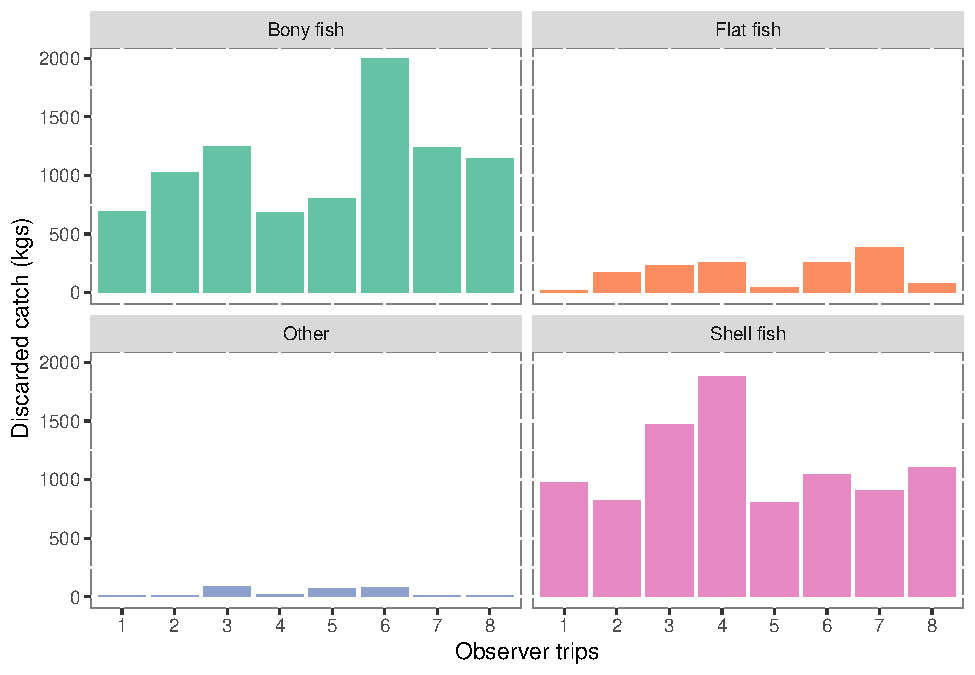
\includegraphics{bookdown-demo_files/figure-latex/unnamed-chunk-5-1} 

}

\caption{Barplots showing a breakdown of weights by species category across fishing trips}\label{fig:unnamed-chunk-5}
\end{figure}

\begin{Shaded}
\begin{Highlighting}[]
\CommentTok{### CODE COMMENTS }\AlertTok{###}
\CommentTok{#[1]. Here the Observerdata is used to get the four categories of species caught and to plot}
\CommentTok{#     them using using four bar plots on a single window using facet_wrap().}
\CommentTok{#[2]. The first argument to ggplot() is the data ("ObserverData"). Then the mapping = aes() where}
\CommentTok{#     the X variable ("TripID") and the Y variable "TotalWeightKG" were supplied. }
\CommentTok{#[3]. The fill argument is used to colour the data by the different categories i.e. "SpeciesCategory2".}
\CommentTok{#[4]. The arguments were passed to geom_bar().}
\CommentTok{#[5]. The plot is formatted using theme() and the legend removed using the legend.position argument. }
\CommentTok{#     Because the names were provide by facet_wrap() a legend would have been redundant. }
\CommentTok{#[6]. X and Y axis labels were added using labs().}
\CommentTok{#[7]. The scale_fill_brewer is used to customize the color of the bars according to the}
\CommentTok{#     species category. The palette argument is used within the function to achieve this. }
\CommentTok{#[8]. facet_wrap() is used to complete the figure.}
\end{Highlighting}
\end{Shaded}

In total 18,608 kgs of fish were landed. Of this amount, bony fish accounted for the highest i.e.~8,804 kgs, followed by shellfish (7,240 kgs), flatfish (1,938 kgs) and others (626 kgs) (Figure 2.1). A similar trend is seen in the mean weights caught per trip for the different categories i.e.~bony fish the highest 1,101 kgs/trip, followed by shell fish (905 kgs/trip), flat fish 242 kgs/trip and Others 78 kgs/trip. The minimum and maximum discard landed by category are as follows: bony fish discards ranged from 683 kgs (trip 4) to 2,410 kgs (trip 6), shell fish from 346 kgs (trip 7) to 1,885 kgs (trip 4), flat fish from 18 kgs (trip 1) to 577 kgs (trip 6) and others from 9 kgs to 257 kgs (trip 6) (Figure 2.1).

\emph{Now we will look at the proportions of the catch discarded}

\hypertarget{proportions-of-the-catch-discarded}{%
\subsection{Proportions of the catch discarded}\label{proportions-of-the-catch-discarded}}

\emph{This will be looked at across fishing trips}

\begin{Shaded}
\begin{Highlighting}[]
\NormalTok{FilteredCatch <-}\StringTok{ }\NormalTok{ObserverData }\OperatorTok\StringTok{ }
\StringTok{  }\KeywordTok{filter}\NormalTok{(CatchCategory }\OperatorTok{==}\StringTok{ "Discarded catch"} \OperatorTok{|}
\StringTok{      }\NormalTok{CatchCategory }\OperatorTok{==}\StringTok{ "Target catch"}\NormalTok{)}

\NormalTok{SumFilteredCatch <-}\StringTok{ }\NormalTok{FilteredCatch }\OperatorTok\StringTok{  }
\StringTok{  }\KeywordTok{group_by}\NormalTok{(TripID, }
\NormalTok{    SpeciesCategory) }\OperatorTok\StringTok{ }
\StringTok{  }\NormalTok{dplyr}\OperatorTok{::}\KeywordTok{summarise}\NormalTok{(}\DataTypeTok{WeightKG =} \KeywordTok{sum}\NormalTok{(TotalWeightKG),}
    \DataTypeTok{.groups =} \StringTok{'drop'}\NormalTok{) }\OperatorTok
\StringTok{  }\KeywordTok{group_by}\NormalTok{(TripID) }\OperatorTok\StringTok{ }
\StringTok{  }\KeywordTok{mutate}\NormalTok{(}\DataTypeTok{Percentage =} \KeywordTok{round}\NormalTok{(}\KeywordTok{prop.table}\NormalTok{(WeightKG)}\OperatorTok{*}\DecValTok{100}\NormalTok{))}

\KeywordTok{ggplot}\NormalTok{(}\DataTypeTok{data =}\NormalTok{ SumFilteredCatch,}
  \DataTypeTok{mapping =} \KeywordTok{aes}\NormalTok{(}\DataTypeTok{x =}\NormalTok{ SpeciesCategory, }
    \DataTypeTok{y =}\NormalTok{ Percentage, }
    \DataTypeTok{fill =}\NormalTok{ SpeciesCategory)) }\OperatorTok{+}
\StringTok{  }\KeywordTok{geom_col}\NormalTok{(}\DataTypeTok{position =} \StringTok{"dodge"}\NormalTok{) }\OperatorTok{+}
\StringTok{  }\KeywordTok{theme}\NormalTok{(}\DataTypeTok{panel.background =} \KeywordTok{element_rect}\NormalTok{(}\DataTypeTok{fill =} \StringTok{"white"}\NormalTok{,}
    \DataTypeTok{colour =} \StringTok{"grey50"}\NormalTok{), }\DataTypeTok{axis.text.x =} \KeywordTok{element_blank}\NormalTok{(), }\DataTypeTok{axis.ticks.x =} \KeywordTok{element_blank}\NormalTok{()) }\OperatorTok{+}
\StringTok{  }\KeywordTok{labs}\NormalTok{(}\DataTypeTok{x=}\StringTok{"Fishing Trips"}\NormalTok{, }
    \DataTypeTok{y =} \StringTok{"Percentages (%)"}\NormalTok{) }\OperatorTok{+}\StringTok{ }
\StringTok{  }\KeywordTok{scale_fill_brewer}\NormalTok{(}\DataTypeTok{palette=}\StringTok{"Set2"}\NormalTok{, }
    \DataTypeTok{name =} \StringTok{" "}\NormalTok{, }
    \DataTypeTok{labels =} \KeywordTok{c}\NormalTok{(}\StringTok{"Discarded catch"}\NormalTok{, }\StringTok{"Target catch"}\NormalTok{)) }\OperatorTok{+}\StringTok{ }\KeywordTok{facet_grid}\NormalTok{(}\OperatorTok{~}\NormalTok{TripID)}
\end{Highlighting}
\end{Shaded}

\begin{figure}

{\centering 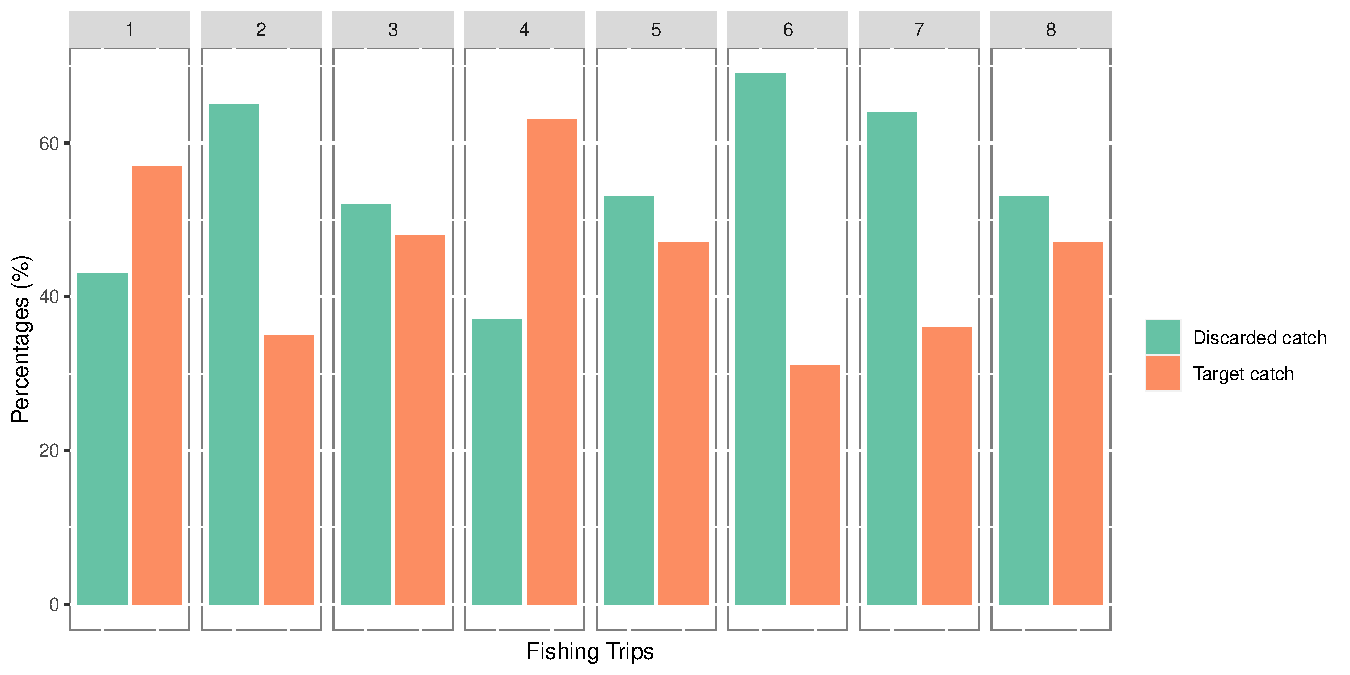
\includegraphics{bookdown-demo_files/figure-latex/unnamed-chunk-6-1} 

}

\caption{Barplot showing a breakdown of weights (proportions) by catch category for the different fishing trips. The numbers at the top of each pair of bars i.e. in the grey area represents the Fishing Trip number ID}\label{fig:unnamed-chunk-6}
\end{figure}

\begin{Shaded}
\begin{Highlighting}[]
\CommentTok{### CODE COMMENTS }\AlertTok{###}
\CommentTok{#[1]. Filtering the observer data by catch category.}
\CommentTok{#[2]. Creating a summary table of weights by fishing trip and species category.}
\CommentTok{#[3]. group_by() and summarise() are used to obtain this along with sum() to create a }
\CommentTok{#     variable called "WeightKG". }
\CommentTok{#[4]. A new variable containing percentages for the different catch categories by }
\CommentTok{#     fishing trips is created using the prop.table() from base R. The values were rounded and }
\CommentTok{#     multiplied by 100 to convert to percentage. }
\CommentTok{#[5]. The differences here is that geom_col() is used here in the place of geom_bar().}
\CommentTok{#     This is used to allow "position" dodge argument which places the catch bars }
\CommentTok{#     side-by-side for easy comparison.}
\CommentTok{#[6]. theme() arguments are similar to "Plot1". The only additions are that the X axis ticks }
\CommentTok{#     and texts were removed using the arguments: axis.ticks.x and axis.text.x, with the }
\CommentTok{#     function value element_blank().}
\CommentTok{#[7]. The scale_fill_brewer is used to customize the color of  the bars according to the catch category.}
\CommentTok{#     The palette argument is used within the function to achieve this. The names argument is used}
\CommentTok{#     to remove the default name and replace with a blank space (" ") and the labels argument }
\CommentTok{#     to add labels to the plot.}
\CommentTok{#[8]. fact_grid() is used to present the data side-by-side by fishing trips. }
\end{Highlighting}
\end{Shaded}

Of the total fish weight, discarded catch accounted for 11,956 kgs (68\%) and target species 5,705 kgs (32\%) (Figure 2.2). Discarded catch proportions (by weight) within the total catch ranged from 37\% (trip 4) to 95\% (trip 6). Target catch on the other hand ranged from 5\% (trip 6) to 63\% (trip 4) (Figure 2.2).

\hypertarget{assessment-summary}{%
\subsection{Assessment summary}\label{assessment-summary}}

The data comprised of four different catch categories: bony fish, shell fish, flat fish and others. From the analysis done bony fish accounted to the highest total weights within the data and least was recorded by the ``others'' category. Discarding of fish species was found to relatively high (i.e.~68\%) when compared to that of the target catch (32\%). With the exception of fishing trip 1 and 4, the total weights of the discarded fish species was always higher than that of the target catch.

\hypertarget{research-question-2}{%
\section{Research Question 2}\label{research-question-2}}

\textbf{What are the species discarded, their relative sampling proportions and weights?}

\hypertarget{species-discarded-and-their-relative-sampling-proportions}{%
\subsection{Species discarded and their relative sampling proportions}\label{species-discarded-and-their-relative-sampling-proportions}}

\begin{Shaded}
\begin{Highlighting}[]
\NormalTok{Table.}\FloatTok{2.1}\NormalTok{ <-}\StringTok{ }\NormalTok{DiscardData }\OperatorTok\StringTok{ }
\StringTok{  }\KeywordTok{group_by}\NormalTok{(OrderTax, }
\NormalTok{           FamilyTax, }
\NormalTok{           LatinNames) }\OperatorTok
\StringTok{  }\NormalTok{dplyr}\OperatorTok{::}\KeywordTok{summarise}\NormalTok{(}\DataTypeTok{n =} \KeywordTok{n}\NormalTok{(), }
                   \DataTypeTok{prop =} \KeywordTok{round}\NormalTok{(n}\OperatorTok{/}\DecValTok{48}\NormalTok{,}\DecValTok{2}\NormalTok{),}
                   \DataTypeTok{.groups =} \StringTok{'drop'}\NormalTok{) }\OperatorTok\StringTok{ }
\StringTok{  }\KeywordTok{arrange}\NormalTok{(OrderTax)}

\NormalTok{Table.}\FloatTok{2.1}\OperatorTok{$}\NormalTok{OrderTax =}\StringTok{ }\KeywordTok{ifelse}\NormalTok{(}\KeywordTok{duplicated}\NormalTok{(Table.}\FloatTok{2.1}\OperatorTok{$}\NormalTok{OrderTax), }\StringTok{""}\NormalTok{,}
\NormalTok{                         Table.}\FloatTok{2.1}\OperatorTok{$}\NormalTok{OrderTax)}
\NormalTok{Table.}\FloatTok{2.1}\OperatorTok{$}\NormalTok{FamilyTax =}\StringTok{ }\KeywordTok{ifelse}\NormalTok{(}\KeywordTok{duplicated}\NormalTok{(Table.}\FloatTok{2.1}\OperatorTok{$}\NormalTok{FamilyTax), }\StringTok{""}\NormalTok{,}
\NormalTok{                          Table.}\FloatTok{2.1}\OperatorTok{$}\NormalTok{FamilyTax)}

\NormalTok{Table.}\FloatTok{2.1} \OperatorTok\StringTok{ }
\StringTok{  }\KeywordTok{kbl}\NormalTok{(}\DataTypeTok{caption =} \StringTok{"Fish taxa identified from the 48 bottom trawl fishing tows sampled off the coast of Guyana. Proportions = species presence in proportion within the total samples."}\NormalTok{,}
    \DataTypeTok{col.names =} \KeywordTok{c}\NormalTok{(}\StringTok{"Orders"}\NormalTok{, }
      \StringTok{"Families"}\NormalTok{, }
      \StringTok{"Scientific names"}\NormalTok{, }
      \StringTok{"Counts"}\NormalTok{,}
      \StringTok{"Proportion"}\NormalTok{),}
    \DataTypeTok{align =} \StringTok{"l"}\NormalTok{) }\OperatorTok
\StringTok{  }\KeywordTok{kable_classic}\NormalTok{() }\OperatorTok
\StringTok{  }\KeywordTok{row_spec}\NormalTok{(}\DecValTok{0}\NormalTok{, }\DataTypeTok{bold =} \OtherTok{TRUE}\NormalTok{) }\OperatorTok
\StringTok{  }\KeywordTok{kable_styling}\NormalTok{(}\DataTypeTok{fixed_thead =}\NormalTok{ T,}
    \DataTypeTok{bootstrap_options =} \KeywordTok{c}\NormalTok{(}\StringTok{"striped"}\NormalTok{,}
      \StringTok{"condensed"}\NormalTok{)) }\OperatorTok\StringTok{ }
\StringTok{  }\KeywordTok{scroll_box}\NormalTok{(}\DataTypeTok{width =} \StringTok{"770px"}\NormalTok{, }\DataTypeTok{height =} \StringTok{"500px"}\NormalTok{)}
\end{Highlighting}
\end{Shaded}

\begin{table}

\caption{\label{tab:unnamed-chunk-7}Fish taxa identified from the 48 bottom trawl fishing tows sampled off the coast of Guyana. Proportions = species presence in proportion within the total samples.}
\centering
\begin{tabular}[t]{l|l|l|l|l}
\hline
\textbf{Orders} & \textbf{Families} & \textbf{Scientific names} & \textbf{Counts} & \textbf{Proportion}\\
\hline
Anguilliformes & Muraenidae & Gymnothorax ocellatus & 1 & 0.02\\
\hline
 & Ophichthidae & Ophichthus gomesii & 37 & 0.77\\
\hline
Batrachoidiformes & Batrachoididae & Batrachoides surinamensis & 34 & 0.71\\
\hline
 &  & Porichthys pauciradiatus & 1 & 0.02\\
\hline
Carcharhiniformes & Triakidae & Mustelus higmani & 6 & 0.12\\
\hline
Clupeiformes & Clupeidae & Harengula jaguana & 27 & 0.56\\
\hline
 & Engraulidae & Anchoa mitchilli & 22 & 0.46\\
\hline
 &  & Anchoa spinifer & 18 & 0.38\\
\hline
 &  & Anchoviella lepidentostole & 1 & 0.02\\
\hline
Decapoda & Aethridae & Hepatus pudibundus & 3 & 0.06\\
\hline
 & Calappidae & Calappa sulcata & 1 & 0.02\\
\hline
 & Diogenidae & Clibanarius foresti & 2 & 0.04\\
\hline
 &  & Petrochirus diogenes & 1 & 0.02\\
\hline
 & Inachoididae & Paulita tuberculata & 3 & 0.06\\
\hline
 & Leucosiidae & Persephona lichtensteinii & 21 & 0.44\\
\hline
 & Malacostraca & Hepatus gronovii & 24 & 0.50\\
\hline
 & Portunidae & Callinectes ornatus & 47 & 0.98\\
\hline
Elopiformes & Elopidae & Elops saurus & 1 & 0.02\\
\hline
Lophiiformes & Ogcocephalidae & Ogcocephalus darwini & 1 & 0.02\\
\hline
Myliobatiformes & Dasyatidae & Dasyatis geijskesi & 6 & 0.12\\
\hline
 &  & Dasyatis guttata & 27 & 0.56\\
\hline
 & Gymnuridae & Gymnura micrura & 31 & 0.65\\
\hline
 & Myliobatidae & Rhinoptera bonasus & 3 & 0.06\\
\hline
 & Urotrygonidae & Urotrygon microphthalmum & 13 & 0.27\\
\hline
Orectolobiformes & Ginglymostomatidae & Ginglymostoma cirratum & 1 & 0.02\\
\hline
Paxillosida & Luidiidae & Luidia senegalensis & 1 & 0.02\\
\hline
Pennatulacea & Renillidae & Renilla muelleri & 2 & 0.04\\
\hline
Perciformes & Carangidae & Chloroscombrus chrysurus & 4 & 0.08\\
\hline
 &  & Selene brownii & 20 & 0.42\\
\hline
 & Centropomidae & Centropomus pectinatus & 4 & 0.08\\
\hline
 &  & Centropomus undecimalis & 1 & 0.02\\
\hline
 & Ephippidae & Chaetodipterus faber & 25 & 0.52\\
\hline
 & Haemulidae & Conodon nobilis & 4 & 0.08\\
\hline
 &  & Genyatremus luteus & 10 & 0.21\\
\hline
 & Sciaenidae & Corvula sanctaeluciae & 2 & 0.04\\
\hline
 &  & Cynoscion jamaicensis & 1 & 0.02\\
\hline
 &  & Cynoscion virescens & 44 & 0.92\\
\hline
 &  & Daysciaena albida & 1 & 0.02\\
\hline
 &  & Larimus breviceps & 21 & 0.44\\
\hline
 &  & Lonchurus elegans & 23 & 0.48\\
\hline
 &  & Macrodon ancylodon & 48 & 1.00\\
\hline
 &  & Micropogonias furnieri & 8 & 0.17\\
\hline
 &  & Nebris microps & 29 & 0.60\\
\hline
 &  & Paralonchurus brasiliensis & 38 & 0.79\\
\hline
 &  & Stellifer microps & 45 & 0.94\\
\hline
 &  & Stellifer rastrifer & 47 & 0.98\\
\hline
 & Scombridae & Scomberomorus brasiliensis & 6 & 0.12\\
\hline
 & Serranidae & Epinephelus flavolimbatus & 4 & 0.08\\
\hline
 & Trichiuridae & Trichiurus lepturus & 42 & 0.88\\
\hline
Pleuronectiformes & Achiridae & Achirus achirus & 38 & 0.79\\
\hline
 & Cynoglossidae & Symphurus plagusia & 43 & 0.90\\
\hline
Polymixiiformes & Polymixiidae & Polymixia lowei & 10 & 0.21\\
\hline
Rajiformes &  & Dasyatis geijskesi & 15 & 0.31\\
\hline
Rhinopristiformes & Rhinobatidae & Pseudobatos percellens & 6 & 0.12\\
\hline
Siluriformes & Ariidae & Arius proops & 14 & 0.29\\
\hline
 &  & Bagre bagre & 42 & 0.88\\
\hline
Stomatopoda & Squillidae & Squilla mantis & 34 & 0.71\\
\hline
Tetraodontiformes & Tetraodontidae & Colomesus psittacus & 23 & 0.48\\
\hline
 &  & Sphoeroides testudineus & 14 & 0.29\\
\hline
Teuthida & Loliginidae & Lolliguncula brevis & 10 & 0.21\\
\hline
Torpediniformes & Narcinidae & Narcine brasiliensis & 11 & 0.23\\
\hline
Unknown & Unknown & Scyphozoa sp. & 25 & 0.52\\
\hline
 &  & Un id & 26 & 0.54\\
\hline
\end{tabular}
\end{table}

\begin{Shaded}
\begin{Highlighting}[]
\CommentTok{### CODE COMMENTS }\AlertTok{###}
\CommentTok{#[1]. group_by() is used create a species Taxonomy table containing the Order, }
\CommentTok{#     Family and Latin/Scientific names. }
\CommentTok{#[2]. A new variable "Proportion" which calculated species proportion based on abundance/count within }
\CommentTok{#     the data is created using summarise().}
\CommentTok{#[3]. The table is arranged by Order. }
\CommentTok{#[4]. ifelse() and duplicated() from base R is used to remove duplicated Order }
\CommentTok{#     and family names from "Table.2.1". This will make the table look less clustered and}
\CommentTok{#     more easily readable. }
\CommentTok{#[5]. All comments here are similar to "Table.1.2"    }
\end{Highlighting}
\end{Shaded}

In total, 61 fish taxa (i.e.~excluding \emph{Scyphozoa sp.} and \emph{Un id}) were identified (Table 2.1), belonging to 39 families in 21 orders, with Perciformes (22 species) being the dominant order. Samples contained between 11 and 31 fish species, with an average of 21 ± 4 species per sample. Four species; \emph{Callinectes ornatus}, \emph{Macrodon ancylodon}, \emph{Stellifer microps} and \emph{Stellifer rastrifer} were the only species present in more than 95\% (45) of the bottom trawl hauls. Otherwise, 20 species were present in more than 50\% of the bottom trawl tows.

\hypertarget{relative-weights-of-discarded-fish-species}{%
\subsection{Relative weights of discarded fish species}\label{relative-weights-of-discarded-fish-species}}

\begin{Shaded}
\begin{Highlighting}[]
\NormalTok{SpeciesWeights <-}\StringTok{ }\NormalTok{DiscardData }\OperatorTok\StringTok{ }
\StringTok{  }\KeywordTok{group_by}\NormalTok{(LatinNames) }\OperatorTok
\StringTok{  }\KeywordTok{filter}\NormalTok{(}\KeywordTok{n}\NormalTok{() }\OperatorTok{>=}\StringTok{ }\DecValTok{5}\NormalTok{) }\OperatorTok\StringTok{ }
\StringTok{  }\KeywordTok{filter}\NormalTok{(TotalWeightKG }\OperatorTok{<}\StringTok{ }\DecValTok{125}\NormalTok{)}


\KeywordTok{ggplot}\NormalTok{(}\DataTypeTok{data =}\NormalTok{ SpeciesWeights,}
  \DataTypeTok{mapping =} \KeywordTok{aes}\NormalTok{(}\DataTypeTok{x =} \KeywordTok{reorder}\NormalTok{(LatinNames,}
\NormalTok{    TotalWeightKG,}
    \DataTypeTok{FUN =}\NormalTok{ median),}
    \DataTypeTok{y =}\NormalTok{ TotalWeightKG)) }\OperatorTok{+}
\StringTok{  }\KeywordTok{geom_boxplot}\NormalTok{() }\OperatorTok{+}
\StringTok{  }\KeywordTok{coord_flip}\NormalTok{()  }\OperatorTok{+}
\StringTok{  }\KeywordTok{labs}\NormalTok{(}\DataTypeTok{x =} \StringTok{"Latin Names"}\NormalTok{,}
    \DataTypeTok{y =}\StringTok{"Weight (kgs)"}\NormalTok{) }\OperatorTok{+}
\StringTok{  }\KeywordTok{theme}\NormalTok{(}\DataTypeTok{panel.background =} \KeywordTok{element_rect}\NormalTok{(}\DataTypeTok{colour =} \StringTok{"White"}\NormalTok{),}
    \DataTypeTok{legend.position =} \StringTok{"none"}\NormalTok{) }\OperatorTok{+}
\StringTok{  }\KeywordTok{theme_bw}\NormalTok{()}
\end{Highlighting}
\end{Shaded}

\begin{figure}

{\centering 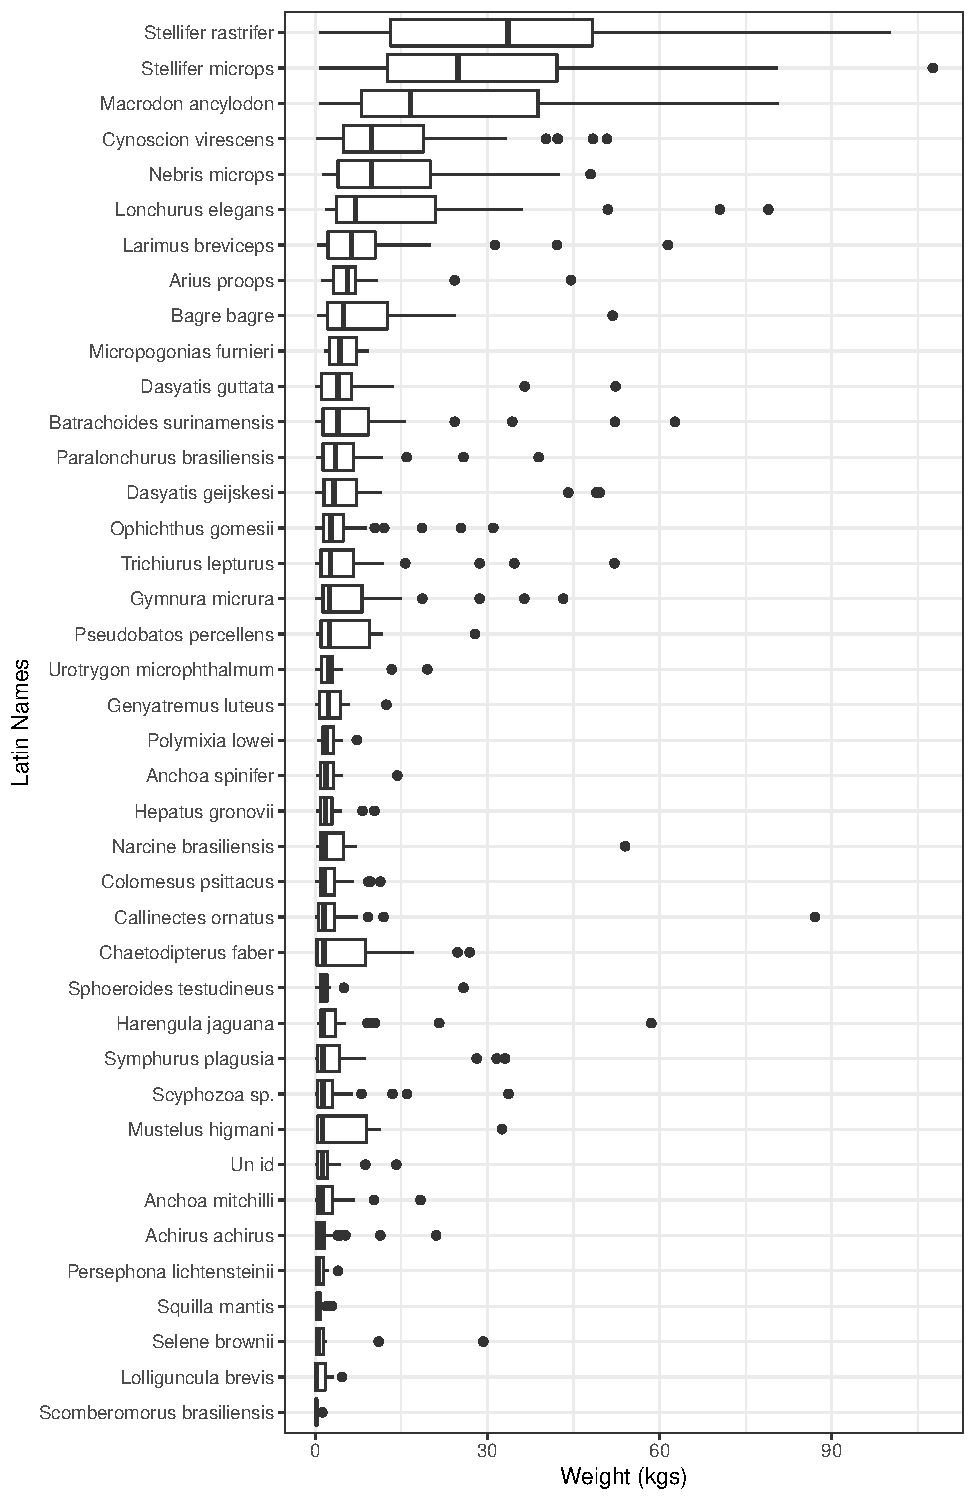
\includegraphics{bookdown-demo_files/figure-latex/unnamed-chunk-8-1} 

}

\caption{Boxplot showing a breakdown of total weight distribution by species. Ranking is done from the highest (top of plot) to the lowest (bottom of plot). Six values above 100 kgs were removed to allow for better visulisation of trends in the species weight distributions.}\label{fig:unnamed-chunk-8}
\end{figure}

\begin{Shaded}
\begin{Highlighting}[]
\CommentTok{### CODE COMMENTS }\AlertTok{###}
\CommentTok{#[1]. First the main data "DiscardData" is filtered to remove species that occurred less than }
\CommentTok{#     five time in sample. This is done using group_by() and filter() from the dplyr package.}
\CommentTok{#     This is done to get meaning summary statistics e.g. median and range. }
\CommentTok{#     The new data is named "SpeciesWeights".   }
\CommentTok{# [2]. The first argument to ggplot() is the data ("SpeciesWeights"). }
\CommentTok{#     Then the mapping = aes() where the X variable ("LatinNames") and the Y variable "TotalWeightKG"}
\CommentTok{#     were supplied. reorder() is used to sort the species from the highest(top of plot) }
\CommentTok{#     to the lowest (bottom of plot) median values.   }
\CommentTok{#[3]. The arguments were passed to geom_boxplot().}
\CommentTok{#[4]. coord_flip() is used to switch the axis to allow for a better presentation of }
\CommentTok{#     the data. This is due to the excess species. }
\CommentTok{#[5]. X and Y axis labels were added using labs().}
\CommentTok{#[6]. The plot is formatted using theme() and the legend removed using the legend.position argument.}
\end{Highlighting}
\end{Shaded}

The data presented in this paragraph and the figure above is filtered to remove those species which occurred less than 5 times in the sample (Figure 2.3). The top five species by median weight landed were: \emph{Polymixia lowei} (18 kgs), followed by \emph{Stellifer rastrifer}, \emph{Stellifer microps}, \emph{Macrodon ancylodon} and \emph{Larimus breviceps} all with 14 kgs, respectively. The weight range for these species are as follows: \emph{Polymixia lowei} (7 to 21 kgs), \emph{Stellifer rastrifer} (1 to 164 kgs), \emph{Stellifer microps} (1 to 133 kgs), \emph{Macrodon ancylodon} (1 to 74 kgs) and \emph{Larimus breviceps} (1 to 61 kgs). The five species with the lowest median weights were: \emph{Mustelus higmani} (1 kg), followed by \emph{Sphoeroides testudineus}, \emph{Persephona lichtensteinii}, \emph{Chaetodipterus faber} and \emph{Hepatus gronovii} all with 2 kgs. The weight range for these species are as follows: \emph{Mustelus higmani} (0.2 to 33 kgs), followed by \emph{Sphoeroides testudineus} (0.1 to 26 kgs), \emph{Persephona lichtensteinii} (0.005 to 14 kgs), \emph{Chaetodipterus faber} (0.01 to 21 kgs) and \emph{Hepatus gronovii} (0.3 to 14 kgs) (Figure 2.3).

\hypertarget{assessment-summary-1}{%
\subsection{Assessment summary}\label{assessment-summary-1}}

From the analysis it was found that 61 different species (i.e.~those positively identified) were discarded (Table 2.1). Of this amount four of them: \emph{Callinectes ornatus}, \emph{Macrodon ancylodon}, \emph{Stellifer microps} and \emph{Stellifer rastrifer} were in at least 45 of the 48 total bottom trawl tows. The latter three fish species, along with \emph{Polymixia lowei} and \emph{Larimus breviceps} were the most dominant species discarded by median weights.

\hypertarget{chapter-2}{%
\chapter{CHAPTER}\label{chapter-2}}

\hypertarget{research-question-3}{%
\section{Research Question 3}\label{research-question-3}}

\textbf{What are the weight distributions of the most common fish species discarded across time of day and fishing depths?}

\hypertarget{weight-distributions-of-the-thirty-30-most-common-fish-species-by-weight-discarded.}{%
\subsection{Weight distributions of the thirty (30) most common fish species (by weight) discarded.}\label{weight-distributions-of-the-thirty-30-most-common-fish-species-by-weight-discarded.}}

\textbf{Data Subsetting}

\begin{Shaded}
\begin{Highlighting}[]
\CommentTok{# Data Subsetting}
\NormalTok{Discard.data <-}\StringTok{ }\NormalTok{ObserverData }\OperatorTok
\StringTok{  }\KeywordTok{filter}\NormalTok{(CatchCategory }\OperatorTok{==}\StringTok{ "Discarded catch"}\NormalTok{)}

\CommentTok{# Viewing all fish species}
\KeywordTok{unique}\NormalTok{(Discard.data}\OperatorTok{$}\NormalTok{LatinNames)}
\end{Highlighting}
\end{Shaded}

\begin{verbatim}
   [1] "Paralonchurus brasiliensis" "Macrodon ancylodon"        
   [3] "Hepatus gronovii"           "Nebris microps"            
   [5] "Bagre bagre"                "Lonchurus elegans"         
   [7] "Stellifer microps"          "Stellifer rastrifer"       
   [9] "Achirus achirus"            "Scyphozoa sp."             
  [11] "Squilla mantis"             "Batrachoides surinamensis" 
  [13] "Cynoscion virescens"        "Gymnothorax ocellatus"     
  [15] "Callinectes ornatus"        "Ophichthus gomesii"        
  [17] "Trichiurus lepturus"        "Persephona lichtensteinii" 
  [19] "Anchoa spinifer"            "Symphurus plagusia"        
  [21] "Colomesus psittacus"        "Micropogonias furnieri"    
  [23] "Rhinoptera bonasus"         "Cynoscion jamaicensis"     
  [25] "Dasyatis guttata"           "Chaetodipterus faber"      
  [27] "Genyatremus luteus"         "Narcine brasiliensis"      
  [29] "Gymnura micrura"            "Pseudobatos percellens"    
  [31] "Selene brownii"             "Harengula jaguana"         
  [33] "Dasyatis geijskesi"         "Lolliguncula brevis"       
  [35] "Un id"                      "Urotrygon microphthalmum"  
  [37] "Ogcocephalus darwini"       "Elops saurus"              
  [39] "Arius proops"               "Scomberomorus brasiliensis"
  [41] "Sphoeroides testudineus"    "Polymixia lowei"           
  [43] "Epinephelus flavolimbatus"  "Larimus breviceps"         
  [45] "Mustelus higmani"           "Chloroscombrus chrysurus"  
  [47] "Hepatus pudibundus"         "Petrochirus diogenes"      
  [49] "Conodon nobilis"            "Corvula sanctaeluciae"     
  [51] "Anchoa mitchilli"           "Renilla muelleri"          
  [53] "Clibanarius foresti"        "Paulita tuberculata"       
  [55] "Daysciaena albida"          "Luidia senegalensis"       
  [57] "Ginglymostoma cirratum"     "Centropomus pectinatus"    
  [59] "Porichthys pauciradiatus"   "Calappa sulcata"           
  [61] "Anchoviella lepidentostole" "Centropomus undecimalis"
\end{verbatim}

\begin{Shaded}
\begin{Highlighting}[]
\CommentTok{### CODE COMMENTS }\AlertTok{###}
\CommentTok{#[1]. Creating a new object named "Discard.data". This object will contain discarded fish species}
\CommentTok{#     only; which is the main focus of this project.}
\CommentTok{#[2]. unique() is used to print the names of all discard fish species from the data. }
\end{Highlighting}
\end{Shaded}

With the exception of \textbf{Un id} which is short for unidentified fish species, a total of 61 different fish species are contained in the discard data. Initially the analysis in this submission will zero in on the more common fish species (by weight) to answer \textbf{Research Question 3} whereas ALL fish species from the data will be utilized in answering \textbf{Research Question 4}.

\textbf{Creating table with the 30 most common fish species discarded}

\begin{Shaded}
\begin{Highlighting}[]
\CommentTok{# Creating Raw Table}
\NormalTok{Table.}\FloatTok{2.1}\NormalTok{ <-}\StringTok{ }\NormalTok{Discard.data }\OperatorTok\StringTok{ }
\StringTok{  }\KeywordTok{group_by}\NormalTok{(LatinNames) }\OperatorTok
\StringTok{  }\NormalTok{dplyr}\OperatorTok{::}\KeywordTok{summarise}\NormalTok{(}\DataTypeTok{Weight.kg =} \KeywordTok{round}\NormalTok{(}\KeywordTok{sum}\NormalTok{(TotalWeightKG),}\DecValTok{2}\NormalTok{),}
    \DataTypeTok{.groups =} \StringTok{"drop"}\NormalTok{) }\OperatorTok\StringTok{ }
\StringTok{  }\NormalTok{dplyr}\OperatorTok{::}\KeywordTok{mutate}\NormalTok{(}\DataTypeTok{Weight.pct =} \KeywordTok{round}\NormalTok{(Weight.kg}\OperatorTok{/}\FloatTok{10055.16}\OperatorTok{*}\DecValTok{100}\NormalTok{,}\DecValTok{2}\NormalTok{)) }\OperatorTok\StringTok{ }
\StringTok{  }\CommentTok{# 10055.16 was calculated manually using formula sum(Table.2.1$Weight.kg).}
\StringTok{  }\KeywordTok{arrange}\NormalTok{(}\KeywordTok{desc}\NormalTok{(Weight.kg)) }\OperatorTok\StringTok{ }
\StringTok{  }\KeywordTok{head}\NormalTok{(}\DecValTok{31}\NormalTok{) }\OperatorTok\StringTok{ }
\StringTok{  }\KeywordTok{filter}\NormalTok{(}\OperatorTok{!}\NormalTok{LatinNames }\OperatorTok{==}\StringTok{ "Un id"}\NormalTok{)}

\CommentTok{# Formatting Table.2.1}
\NormalTok{Table.}\FloatTok{2.1} \OperatorTok
\StringTok{  }\KeywordTok{kbl}\NormalTok{(}\DataTypeTok{caption =} \StringTok{"The top 30 fish species by total weights (kgs) caught."}\NormalTok{) }\OperatorTok
\StringTok{  }\KeywordTok{kable_classic}\NormalTok{() }\OperatorTok
\StringTok{  }\KeywordTok{row_spec}\NormalTok{(}\DecValTok{0}\NormalTok{, }\DataTypeTok{bold =} \OtherTok{TRUE}\NormalTok{) }\OperatorTok
\StringTok{  }\KeywordTok{kable_styling}\NormalTok{(}\DataTypeTok{fixed_thead =}\NormalTok{ T,}
    \DataTypeTok{bootstrap_options =} \KeywordTok{c}\NormalTok{(}\StringTok{"striped"}\NormalTok{,}
      \StringTok{"condensed"}\NormalTok{)) }\OperatorTok\StringTok{ }
\StringTok{  }\KeywordTok{scroll_box}\NormalTok{(}\DataTypeTok{width =} \StringTok{"770px"}\NormalTok{, }\DataTypeTok{height =} \StringTok{"500px"}\NormalTok{)}
\end{Highlighting}
\end{Shaded}

\begin{table}

\caption{\label{tab:unnamed-chunk-10}The top 30 fish species by total weights (kgs) caught.}
\centering
\begin{tabular}[t]{l|r|r}
\hline
\textbf{LatinNames} & \textbf{Weight.kg} & \textbf{Weight.pct}\\
\hline
Stellifer rastrifer & 1734.77 & 17.25\\
\hline
Stellifer microps & 1440.64 & 14.33\\
\hline
Macrodon ancylodon & 1226.92 & 12.20\\
\hline
Cynoscion virescens & 637.26 & 6.34\\
\hline
Trichiurus lepturus & 469.85 & 4.67\\
\hline
Nebris microps & 409.90 & 4.08\\
\hline
Lonchurus elegans & 409.10 & 4.07\\
\hline
Bagre bagre & 375.99 & 3.74\\
\hline
Dasyatis geijskesi & 363.81 & 3.62\\
\hline
Symphurus plagusia & 357.44 & 3.55\\
\hline
Batrachoides surinamensis & 313.17 & 3.11\\
\hline
Larimus breviceps & 245.26 & 2.44\\
\hline
Gymnura micrura & 227.69 & 2.26\\
\hline
Paralonchurus brasiliensis & 217.28 & 2.16\\
\hline
Callinectes ornatus & 198.55 & 1.97\\
\hline
Dasyatis guttata & 187.56 & 1.87\\
\hline
Ophichthus gomesii & 184.89 & 1.84\\
\hline
Harengula jaguana & 147.03 & 1.46\\
\hline
Chaetodipterus faber & 136.11 & 1.35\\
\hline
Arius proops & 126.26 & 1.26\\
\hline
Scyphozoa sp. & 104.46 & 1.04\\
\hline
Narcine brasiliensis & 78.61 & 0.78\\
\hline
Achirus achirus & 73.55 & 0.73\\
\hline
Colomesus psittacus & 67.94 & 0.68\\
\hline
Anchoa mitchilli & 59.97 & 0.60\\
\hline
Hepatus gronovii & 59.91 & 0.60\\
\hline
Urotrygon microphthalmum & 54.58 & 0.54\\
\hline
Selene brownii & 53.54 & 0.53\\
\hline
Mustelus higmani & 46.96 & 0.47\\
\hline
Anchoa spinifer & 46.16 & 0.46\\
\hline
\end{tabular}
\end{table}

\begin{Shaded}
\begin{Highlighting}[]
\CommentTok{### CODE COMMENTS }\AlertTok{###}
\CommentTok{#[1]. The name of the table object is Table.2.1 }
\CommentTok{#[2]. group_by() is used to group the data by Latin Names.}
\CommentTok{#[3]. summarise() is called directly from the dplyr package using the command "package name::function" }
\CommentTok{#     due to clashes with other loaded R packages.}
\CommentTok{#[3.1]. summarise() is then used to create a new variable called "Weight.kg". "Weight.kg" }
\CommentTok{#       contains the summed weights for each discarded fish species. }
\CommentTok{#[3.2]. The ".group" argument is used to control the grouping structure of the output, which }
\CommentTok{#       in this case it was dropped. }
\CommentTok{#[4]. mutate() from the dplyr package is used to create a variable: "Weight.pct" i.e. Short for }
\CommentTok{#     weight percentage. }
\CommentTok{#[4.1]. Strangely I was not getting percentage to add up to 100% when I used the formula }
\CommentTok{#       (Weight.kg/sum(Weight.kg)*100), so instead I did it manually.}
\CommentTok{#[4.2]. "Weight.pct" was rounded to 2 decimal places using round(). }
\CommentTok{#[5]. The table is sorted by the "Weight" variable in descending order using arrange(desc()). }
\CommentTok{#[6]. head() is used to select the first 31 rows/fish species.}
\CommentTok{#[7]. filter() is used to remove "Un id" which  refers to multiple fish species that were unidentified }
\CommentTok{#     and not a single fish species.}
\CommentTok{#[8]. kbl() from the kableExtra package is used as the primary formatting source for "Table.2.1" to }
\CommentTok{#     solve the auto format setting in a better way.}
\CommentTok{#[9]. kable_classic() is used to set the theme. }
\CommentTok{#[10]. row_spec() is used to select and bold the column texts.}
\CommentTok{#[11]. kable_styling() is used to freeze the table headers and to adjust the theme and appearance of "Table.2.1".}
\end{Highlighting}
\end{Shaded}

The total weight of the 30 fish species examined in Table 2.1 was 10,055 kgs. From the table we see that three fish species only: \emph{Stellifer rastrifer}(17.25 \%), \emph{Stellifer microps}(14.33 \%) and \emph{Macrodon ancylodon} (12.20) were responsible for (43.78 \%) of total weight. These fish species individually accounted for more than 10\% of the weights. This is quite substantial consider that they collectively were just 10 \% of all the fish species examined. Some of the other more common fish species by weight discarded were \emph{Cynoscion virescens}(6.34 \%), \emph{Trichiurus lepturus}(4.67 \%), \emph{Nebris microps}(4.08 \%), \emph{Lonchurus elegans}(4.07 \%), \emph{Bagre bagre}(3.74 \%), \emph{Dasyatis geijskesi}(3.62 \%) and \emph{Symphurus plagusia}(3.55 \%).

\hypertarget{subsetting-the-top-6-most-common-fish-species-by-weight}{%
\subsection{Subsetting the top 6 most common fish species by weight}\label{subsetting-the-top-6-most-common-fish-species-by-weight}}

\textbf{Inspection of the data before analysis}

\begin{Shaded}
\begin{Highlighting}[]
\CommentTok{# Creating a vector }
\NormalTok{Top.}\FloatTok{6.}\NormalTok{fish.names <-}\StringTok{ }\KeywordTok{head}\NormalTok{(Table.}\FloatTok{2.1}\OperatorTok{$}\NormalTok{LatinNames, }\DecValTok{6}\NormalTok{) }

\CommentTok{# Filtering data}
\NormalTok{Top.}\FloatTok{6.}\NormalTok{fish.data <-}\StringTok{ }\NormalTok{DiscardData }\OperatorTok\StringTok{ }
\StringTok{  }\KeywordTok{filter}\NormalTok{(LatinNames }\OperatorTok\StringTok{ }\NormalTok{Top.}\FloatTok{6.}\NormalTok{fish.names) }

\CommentTok{# Plotting data}
\KeywordTok{ggplot}\NormalTok{(}\DataTypeTok{data =}\NormalTok{ Top.}\FloatTok{6.}\NormalTok{fish.data,}
  \DataTypeTok{mapping =} \KeywordTok{aes}\NormalTok{(}\DataTypeTok{x =}\NormalTok{ DragID2,}
    \DataTypeTok{y =}\NormalTok{ TotalWeightKG)) }\OperatorTok{+}
\StringTok{  }\KeywordTok{geom_point}\NormalTok{(}\DataTypeTok{alpha =} \FloatTok{0.5}\NormalTok{) }\OperatorTok{+}
\StringTok{  }\KeywordTok{theme_bw}\NormalTok{() }\OperatorTok{+}
\StringTok{  }\KeywordTok{labs}\NormalTok{(}\DataTypeTok{x =} \StringTok{"Bottom trawl fishing tows"}\NormalTok{,}
    \DataTypeTok{y =} \StringTok{"Weight (kgs)"}\NormalTok{,}
    \DataTypeTok{title =} \StringTok{"Figure 2.1: Scatter plot of discarded fish species weights against }\CharTok{\textbackslash{}n}\StringTok{bottom trawl fishing tows"}\NormalTok{,}
    \DataTypeTok{subtitle =} \StringTok{"A total of 48 bottom trawl fishing tows were made }\CharTok{\textbackslash{}n}\StringTok{Most of the weight observations are below 125 kgs"}\NormalTok{)}
\end{Highlighting}
\end{Shaded}

\begin{center}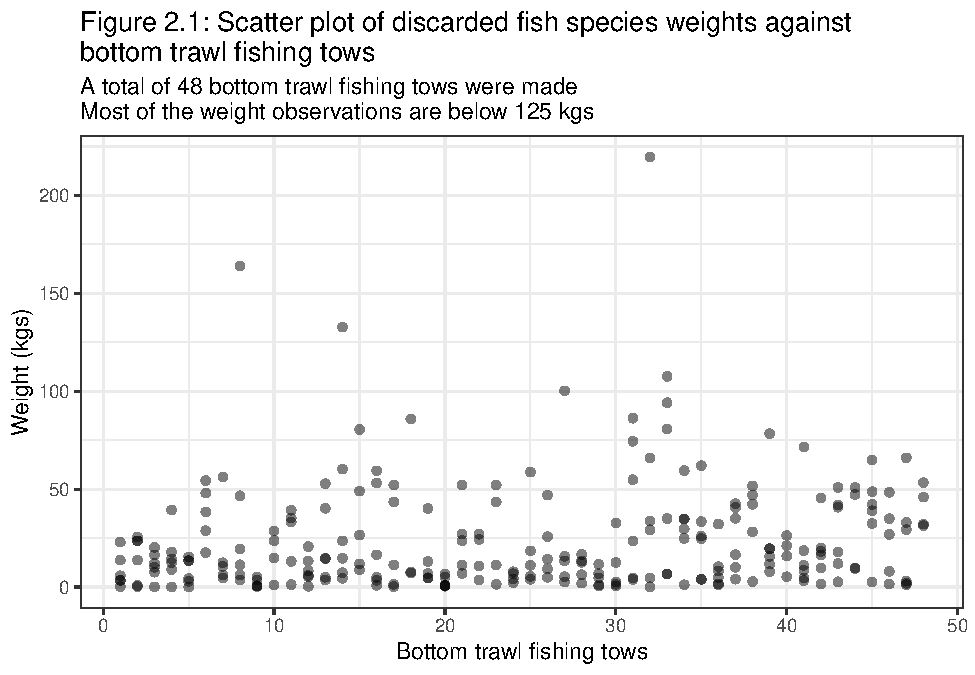
\includegraphics{bookdown-demo_files/figure-latex/unnamed-chunk-11-1} \end{center}

\begin{Shaded}
\begin{Highlighting}[]
\CommentTok{### CODE COMMENTS }\AlertTok{###}
\CommentTok{#[1]. The vector "Top.6.fish.names" is created using head(). The fish species names were }
\CommentTok{#     extracted from the "Table.2.1" object. }
\CommentTok{#[2]. The "DiscardData" data is subsetted to remove the observations for the top 6 fish species. }
\CommentTok{#     The new object is called "Top.6.fish.data". This is done using filter().}
\CommentTok{#[3]. The first argument to ggplot() is the new data "Top.6.fish.data". }
\CommentTok{#[3.1]. The x-variable "DragID2" and the y-variable "TotalWeightKG" are supplied to mapping = aes().   }
\CommentTok{#[4]. The arguments are passed to geom_point(). Transparency of the points were set at "0.5" using alpha().}
\CommentTok{#     This makes the over-plotted points more visible. geom_jitter() was another option but the points }
\CommentTok{#     in this case was not many.     }
\CommentTok{#[5]. The plot theme is set with theme_bw(). }
\CommentTok{#[6]. The x, y, title and subtitle labels are added using labs().}
\end{Highlighting}
\end{Shaded}

After seeing the top 30 fish species by weight in \emph{Table 2.1} we will now zoom in on the top 6 fish species. Before any analysis it is important to inspect the data visually. From the scatter plot (Figure 2.1), we see that for the 48 bottom trawl fishing tows conducted, the weights ranged between 0.018 kgs to 219.586 kgs. Despite this range most of the points were below 125 kgs. This means that a few data points were \emph{abnormally high}. These points are highlighted below and will subsequently be removed from the analysis, as they were probably mistakes. This decision was guided by my knowledge about the data.

\textbf{Visualizing outliers}

\begin{Shaded}
\begin{Highlighting}[]
\CommentTok{# Subsetting data with outliers}
\NormalTok{Outliers <-}\StringTok{ }\NormalTok{Top.}\FloatTok{6.}\NormalTok{fish.data }\OperatorTok\StringTok{ }
\StringTok{  }\KeywordTok{filter}\NormalTok{(TotalWeightKG }\OperatorTok{>}\StringTok{ }\DecValTok{125}\NormalTok{) }

\CommentTok{# Plotting data}
\KeywordTok{ggplot}\NormalTok{(}\DataTypeTok{data =}\NormalTok{ Top.}\FloatTok{6.}\NormalTok{fish.data) }\OperatorTok{+}
\StringTok{  }\KeywordTok{geom_point}\NormalTok{(}\KeywordTok{aes}\NormalTok{(}\DataTypeTok{x =}\NormalTok{ DragID2,}
    \DataTypeTok{y =}\NormalTok{ TotalWeightKG), }
    \DataTypeTok{alpha =} \FloatTok{0.5}\NormalTok{) }\OperatorTok{+}
\StringTok{  }\KeywordTok{geom_point}\NormalTok{(}\DataTypeTok{data =}\NormalTok{ Outliers,}
    \KeywordTok{aes}\NormalTok{(}\DataTypeTok{x =}\NormalTok{ DragID2,}
      \DataTypeTok{y =}\NormalTok{ TotalWeightKG,}
      \DataTypeTok{color =}\NormalTok{ LatinNames), }
    \DataTypeTok{size =} \DecValTok{3}\NormalTok{) }\OperatorTok{+}
\StringTok{  }\KeywordTok{theme_bw}\NormalTok{() }\OperatorTok{+}
\StringTok{  }\KeywordTok{theme}\NormalTok{(}\DataTypeTok{legend.position =} \StringTok{"bottom"}\NormalTok{,}
    \DataTypeTok{legend.title =} \KeywordTok{element_blank}\NormalTok{()) }\OperatorTok{+}
\StringTok{  }\KeywordTok{guides}\NormalTok{(}\DataTypeTok{color =} \KeywordTok{guide_legend}\NormalTok{(}\DataTypeTok{title =} \StringTok{"Latin Names"}\NormalTok{)) }\OperatorTok{+}
\StringTok{  }\KeywordTok{labs}\NormalTok{(}\DataTypeTok{x =} \StringTok{"Bottom trawl fishing tows"}\NormalTok{,}
    \DataTypeTok{y =} \StringTok{"Weight (kgs)"}\NormalTok{,}
    \DataTypeTok{title =} \StringTok{"Figure 2.2: Scatter plot of discarded fish species weights against }\CharTok{\textbackslash{}n}\StringTok{bottom trawl fishing tows"}\NormalTok{,}
    \DataTypeTok{subtitle =} \StringTok{"The oservations above 125 kgs removed - possible outliers }\CharTok{\textbackslash{}n}\StringTok{ Points on the plot represent discarded fish species"}\NormalTok{)}
\end{Highlighting}
\end{Shaded}

\begin{center}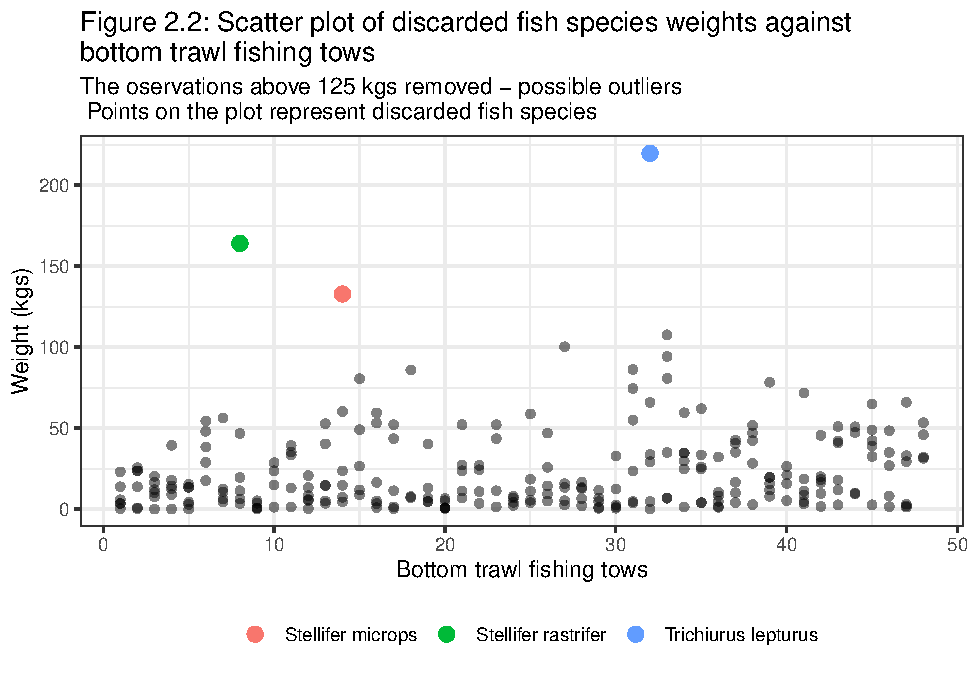
\includegraphics{bookdown-demo_files/figure-latex/unnamed-chunk-12-1} \end{center}

\begin{Shaded}
\begin{Highlighting}[]
\CommentTok{### CODE COMMENTS }\AlertTok{###}
\CommentTok{#[1]. The "Top.6.fish.data" data is subsetted to remove the outlier observations. The new object }
\CommentTok{#     is called "Outliers". This is done using filter(). }
\CommentTok{#[2]. The comments for the code used to produce Figure 2.2 is similar to that for Figure 2.1, }
\CommentTok{#     except for the following:}
\CommentTok{#[2.1]. geom_point() was used twice with the two different data. The second data "Outliers" was used with }
\CommentTok{#       size() and color() arguments to make the outliers visible.}
\CommentTok{#[2.2]. legend.position() argument was used in theme() to show the legend to the bottom.}
\CommentTok{#[2.3]. The name of the legend was specified using guides(). }
\end{Highlighting}
\end{Shaded}

From Figure 2.2 we see that there were three abnormally high data points. These were for discarded fish species \emph{Stellifer microps}(pink), \emph{Stellifer rastrifer}(green) and \emph{Trichiurus lepturus}(blue). As mentioned before these points are strangely high and therefore are perceived to be incorrectly entered and thus will be omitted from the analysis.

\hypertarget{assessment-of-fish-species-against-time-of-day}{%
\subsection{Assessment of fish species against time of day}\label{assessment-of-fish-species-against-time-of-day}}

\hypertarget{weight-distributions-for-the-six-6-most-common-fish-species-by-weights-discarded-across-time-of-day.}{%
\subsubsection{Weight distributions for the Six (6) most common fish species (by weights) discarded across time of day.}\label{weight-distributions-for-the-six-6-most-common-fish-species-by-weights-discarded-across-time-of-day.}}

\begin{Shaded}
\begin{Highlighting}[]
\CommentTok{# Removing the outliers}
\NormalTok{Top.}\FloatTok{6.}\NormalTok{fish.data <-}\StringTok{ }\NormalTok{Top.}\FloatTok{6.}\NormalTok{fish.data }\OperatorTok\StringTok{ }
\StringTok{  }\KeywordTok{filter}\NormalTok{(TotalWeightKG }\OperatorTok{<}\StringTok{ }\DecValTok{125}\NormalTok{)}

\CommentTok{# Plotting data}
\KeywordTok{ggplot}\NormalTok{(Top.}\FloatTok{6.}\NormalTok{fish.data,}
  \KeywordTok{aes}\NormalTok{(}\DataTypeTok{x =}\NormalTok{ LatinNames, }
    \DataTypeTok{y =}\NormalTok{ TotalWeightKG, }
    \DataTypeTok{colour =}\NormalTok{ LatinNames)) }\OperatorTok{+}
\StringTok{  }\KeywordTok{geom_boxplot}\NormalTok{(}\DataTypeTok{alpha =} \FloatTok{0.5}\NormalTok{) }\OperatorTok{+}
\StringTok{  }\KeywordTok{stat_boxplot}\NormalTok{(}\DataTypeTok{geom =} \StringTok{'errorbar'}\NormalTok{, }\DataTypeTok{width =} \FloatTok{0.2}\NormalTok{) }\OperatorTok{+}
\StringTok{  }\KeywordTok{theme_bw}\NormalTok{() }\OperatorTok{+}
\StringTok{  }\KeywordTok{theme}\NormalTok{(}\DataTypeTok{panel.background =} \KeywordTok{element_rect}\NormalTok{(}\DataTypeTok{fill =} \StringTok{"white"}\NormalTok{,}
    \DataTypeTok{colour =} \StringTok{"grey50"}\NormalTok{),}
    \DataTypeTok{axis.text.x =} \KeywordTok{element_blank}\NormalTok{(),}
    \DataTypeTok{axis.ticks.x =} \KeywordTok{element_blank}\NormalTok{(),}
    \DataTypeTok{legend.title =} \KeywordTok{element_blank}\NormalTok{(),}
    \DataTypeTok{legend.position =} \StringTok{"bottom"}\NormalTok{) }\OperatorTok{+}
\StringTok{  }\KeywordTok{labs}\NormalTok{(}\DataTypeTok{x =} \StringTok{"Latin Names"}\NormalTok{,}
    \DataTypeTok{y =} \StringTok{"Weight (kgs)"}\NormalTok{,}
    \DataTypeTok{title =} \StringTok{"Figure 2.3: Boxplot of discarded fish species weights by time of day"}\NormalTok{,}
    \DataTypeTok{subtitle =} \StringTok{"Colours are used to represent the different fish species"}\NormalTok{) }\OperatorTok{+}
\StringTok{  }\KeywordTok{facet_wrap}\NormalTok{(}\OperatorTok{~}\NormalTok{TimePeriods,}
    \DataTypeTok{ncol =} \DecValTok{2}\NormalTok{)}
\end{Highlighting}
\end{Shaded}

\begin{center}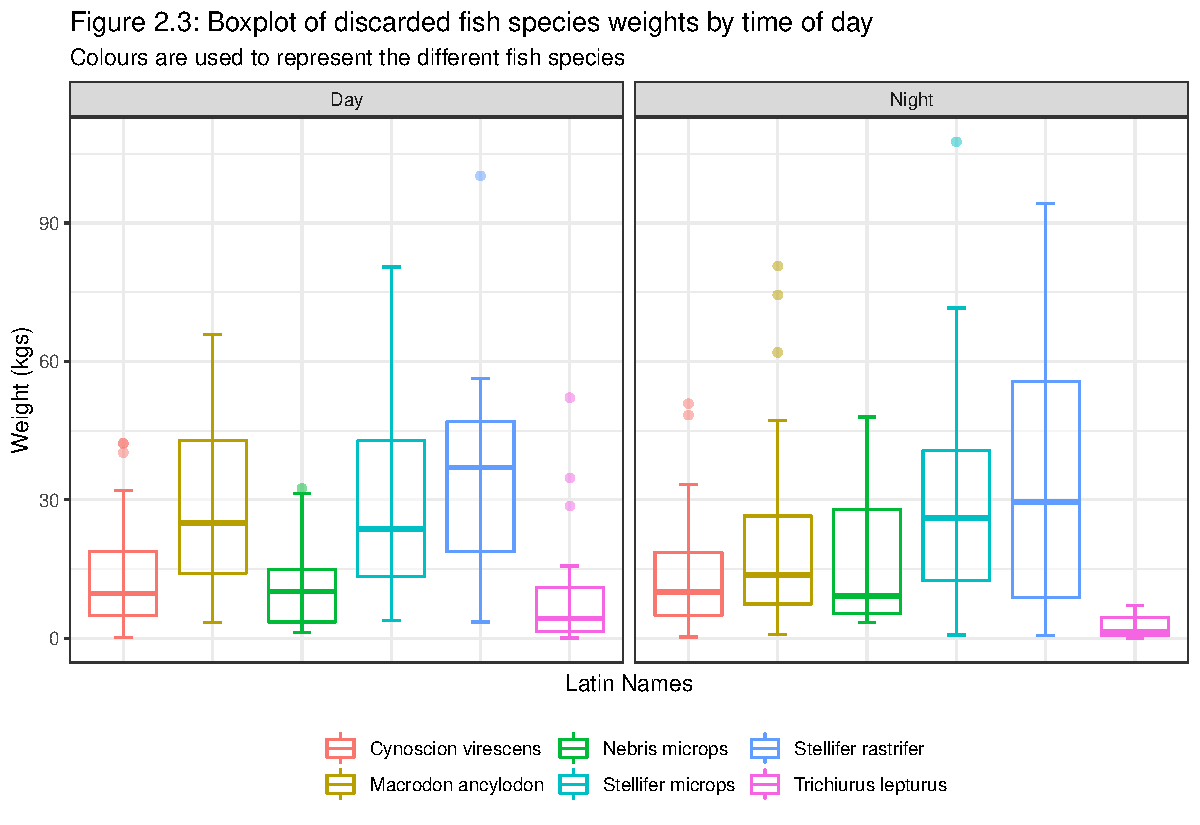
\includegraphics{bookdown-demo_files/figure-latex/unnamed-chunk-13-1} \end{center}

\begin{Shaded}
\begin{Highlighting}[]
\CommentTok{### CODE COMMENTS }\AlertTok{###}
\CommentTok{#[1]. The "Top.6.fish.data" data is subsetted to remove the three outlier values. The name is }
\CommentTok{#     maintained for the new object. This is done using filter().}
\CommentTok{#[2]. The first argument to ggplot() is the data "Top.6.fish.data". }
\CommentTok{#[2.1]. The x-variable "LatinNames" and the y-variable "TotalWeightKG" are supplied to mapping = aes(). }
\CommentTok{#[2.1.1] The fish species are colored using color() within mapping = aes().     }
\CommentTok{#[3]. Box plots are created using geom_boxplot.}
\CommentTok{#[4]. stat_boxplot() is used to format the error bars at the minimum and maximum points on the whisker. }
\CommentTok{#[5]. theme() in this instance was also used to remove the axis tick marks to make the graph look less clustered. }
\CommentTok{#[6]. The data was grouped using facet_wrap() with 2 columns (i.e. ncol = 2).   }
\end{Highlighting}
\end{Shaded}

\textbf{Creating a table with the top 6 fish species across time-periods}

\begin{Shaded}
\begin{Highlighting}[]
\CommentTok{# Creating table}
\NormalTok{Table.}\FloatTok{2.2}\NormalTok{ <-}\StringTok{ }\NormalTok{Top.}\FloatTok{6.}\NormalTok{fish.data }\OperatorTok\StringTok{ }
\StringTok{  }\KeywordTok{group_by}\NormalTok{(LatinNames,}
\NormalTok{    TimePeriods) }\OperatorTok\StringTok{ }
\StringTok{  }\NormalTok{dplyr}\OperatorTok{::}\KeywordTok{summarise}\NormalTok{(}\DataTypeTok{SumWeights =} \KeywordTok{round}\NormalTok{(}\KeywordTok{sum}\NormalTok{(TotalWeightKG)),}
    \DataTypeTok{MedianWeights =} \KeywordTok{round}\NormalTok{(}\KeywordTok{median}\NormalTok{(TotalWeightKG)),}
    \DataTypeTok{.groups =} \StringTok{'drop'}\NormalTok{)}

\CommentTok{# Printing table}
\NormalTok{Table.}\FloatTok{2.2} \OperatorTok\StringTok{ }
\StringTok{  }\KeywordTok{kbl}\NormalTok{(}\DataTypeTok{caption =} \StringTok{"The top 6 fish species by total weights (kgs) caught across time of day"}\NormalTok{) }\OperatorTok
\StringTok{  }\KeywordTok{kable_classic}\NormalTok{(}\StringTok{"striped"}\NormalTok{) }\OperatorTok\StringTok{ }
\StringTok{  }\KeywordTok{row_spec}\NormalTok{(}\DecValTok{0}\NormalTok{, }\DataTypeTok{bold =} \OtherTok{TRUE}\NormalTok{) }\OperatorTok\StringTok{ }
\StringTok{  }\KeywordTok{column_spec}\NormalTok{(}\DecValTok{1}\NormalTok{, }\DataTypeTok{bold =}\NormalTok{ T) }\OperatorTok\StringTok{ }
\StringTok{  }\KeywordTok{kable_styling}\NormalTok{(}\DataTypeTok{fixed_thead =}\NormalTok{ T,}
    \DataTypeTok{bootstrap_options =} \StringTok{"condensed"}\NormalTok{) }
\end{Highlighting}
\end{Shaded}

\begin{table}

\caption{\label{tab:unnamed-chunk-14}The top 6 fish species by total weights (kgs) caught across time of day}
\centering
\begin{tabular}[t]{>{}l|l|r|r}
\hline
\textbf{LatinNames} & \textbf{TimePeriods} & \textbf{SumWeights} & \textbf{MedianWeights}\\
\hline
\textbf{Cynoscion virescens} & Day & 328 & 10\\
\hline
\textbf{Cynoscion virescens} & Night & 310 & 10\\
\hline
\textbf{Macrodon ancylodon} & Day & 703 & 25\\
\hline
\textbf{Macrodon ancylodon} & Night & 524 & 14\\
\hline
\textbf{Nebris microps} & Day & 170 & 10\\
\hline
\textbf{Nebris microps} & Night & 240 & 9\\
\hline
\textbf{Stellifer microps} & Day & 673 & 24\\
\hline
\textbf{Stellifer microps} & Night & 634 & 26\\
\hline
\textbf{Stellifer rastrifer} & Day & 765 & 37\\
\hline
\textbf{Stellifer rastrifer} & Night & 806 & 30\\
\hline
\textbf{Trichiurus lepturus} & Day & 196 & 4\\
\hline
\textbf{Trichiurus lepturus} & Night & 54 & 1\\
\hline
\end{tabular}
\end{table}

\begin{Shaded}
\begin{Highlighting}[]
\CommentTok{### CODE COMMENTS }\AlertTok{###}
\CommentTok{#[1]. To see a description of the functions used in this code and how they work please refer }
\CommentTok{#     to the code comments made at Table.2.1}
\end{Highlighting}
\end{Shaded}

Of the total discard fish species weights (5,403 kgs) for the top 6 fish species, 52\% (2,835 kgs) were recorded for the day and 48\% (2,568 kgs) from the night (Table 2.2). This means that the cumulative fish species weights were marginally higher in the day when compared to the night. Further, we see that the total weights by fish species in the day ranged from 170 kgs(\emph{Nebris microps}) to 765 kgs(\emph{Stellifer rastrifer}). Whereas the total weights in the night ranged from 54 kgs (\emph{Trichiurus lepturus}) to 806 kgs (\emph{Stellifer rastrifer}). From Figure 2.3 and Table 2.2 we see that \emph{Trichiurus lepturus} had the lowest median weights across time of day i.e.~4 kgs (day) and 1 kg (night) for the top 6 fish species examined. While \emph{Stellifer rastrifer} recorded the highest median weights for both the day (37 kgs) and night (30 kgs). Therefore, we can conclude that \emph{Stellifer rastrifer} was the most dominant discarded fish species across time of day with the highest individual total weight and median, while \emph{Nebris microps} and \emph{Trichiurus lepturus} were the least dominant discarded fish species i.e.~recording the lowest total weight and median, respectively, across time of day.

\hypertarget{assessment-of-fish-species-against-fishing-depths}{%
\subsection{Assessment of fish species against fishing depths}\label{assessment-of-fish-species-against-fishing-depths}}

\hypertarget{box-plot-showing-the-weight-distribution-for-the-six-6-most-common-fish-species-by-weight-discarded-across-fishing-depths.}{%
\subsubsection{Box plot showing the weight distribution for the six (6) most common fish species (by weight) discarded across fishing depths.}\label{box-plot-showing-the-weight-distribution-for-the-six-6-most-common-fish-species-by-weight-discarded-across-fishing-depths.}}

\begin{Shaded}
\begin{Highlighting}[]
\KeywordTok{ggplot}\NormalTok{(Top.}\FloatTok{6.}\NormalTok{fish.data,}
  \KeywordTok{aes}\NormalTok{(}\DataTypeTok{x =}\NormalTok{ LatinNames, }
    \DataTypeTok{y =}\NormalTok{ TotalWeightKG, }
    \DataTypeTok{colour =}\NormalTok{ LatinNames)) }\OperatorTok{+}
\StringTok{  }\KeywordTok{geom_boxplot}\NormalTok{(}\DataTypeTok{alpha =} \FloatTok{0.5}\NormalTok{) }\OperatorTok{+}\StringTok{ }
\StringTok{  }\KeywordTok{stat_boxplot}\NormalTok{(}\DataTypeTok{geom =} \StringTok{'errorbar'}\NormalTok{, }\DataTypeTok{width =} \FloatTok{0.2}\NormalTok{) }\OperatorTok{+}
\StringTok{  }\KeywordTok{theme_bw}\NormalTok{() }\OperatorTok{+}
\StringTok{  }\KeywordTok{theme}\NormalTok{(}\DataTypeTok{panel.background =} \KeywordTok{element_rect}\NormalTok{(}\DataTypeTok{fill =} \StringTok{"white"}\NormalTok{,}
    \DataTypeTok{colour =} \StringTok{"grey50"}\NormalTok{),}
    \DataTypeTok{axis.text.x =} \KeywordTok{element_blank}\NormalTok{(),}
    \DataTypeTok{axis.ticks.x =} \KeywordTok{element_blank}\NormalTok{(),}
    \DataTypeTok{legend.title =} \KeywordTok{element_blank}\NormalTok{(),}
    \DataTypeTok{legend.position =} \StringTok{"bottom"}\NormalTok{)  }\OperatorTok{+}
\StringTok{  }\KeywordTok{labs}\NormalTok{(}\DataTypeTok{x =} \StringTok{"Fish Species"}\NormalTok{,}
    \DataTypeTok{y =} \StringTok{"Weights (kgs)"}\NormalTok{,}
    \DataTypeTok{title =} \StringTok{"Figure 2.4: Boxplot of discarded fish species weights by fishing depths"}\NormalTok{,}
    \DataTypeTok{subtitle =} \StringTok{"Colours are used to represent the different fish species"}\NormalTok{) }\OperatorTok{+}
\StringTok{  }\KeywordTok{facet_wrap}\NormalTok{(.}\OperatorTok{~}\NormalTok{FishingDepth2) }
\end{Highlighting}
\end{Shaded}

\begin{center}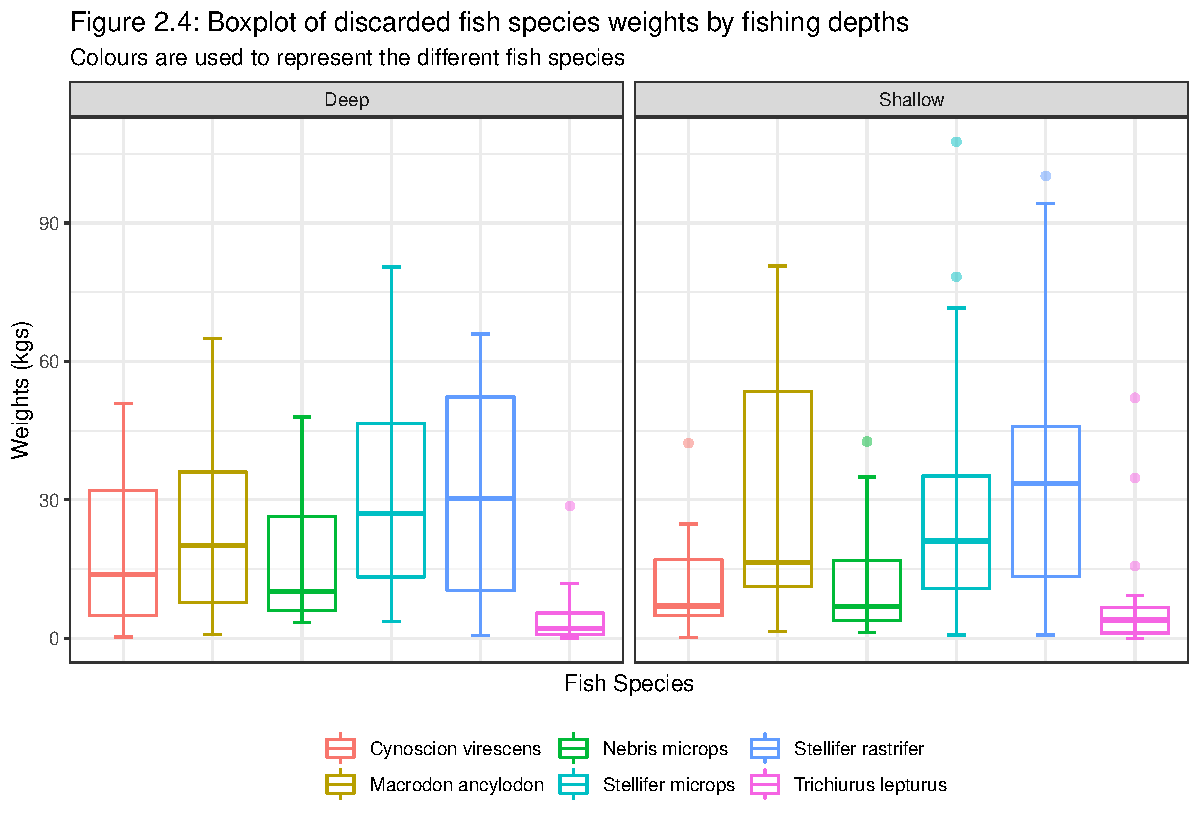
\includegraphics{bookdown-demo_files/figure-latex/unnamed-chunk-15-1} \end{center}

\begin{Shaded}
\begin{Highlighting}[]
\CommentTok{### CODE COMMENTS }\AlertTok{###}
\CommentTok{#[1]. To see a description of what the functions in this code are doing please refer to the }
\CommentTok{#     code comments made at Figure 2.3. The only exception being that time-period is replaced by fishing depths.  }
\end{Highlighting}
\end{Shaded}

\textbf{Creating a table of the top 6 fish species across fishing depths}

\begin{Shaded}
\begin{Highlighting}[]
\NormalTok{Table.}\FloatTok{2.3}\NormalTok{ <-}\StringTok{ }\NormalTok{Top.}\FloatTok{6.}\NormalTok{fish.data }\OperatorTok\StringTok{ }
\StringTok{  }\KeywordTok{group_by}\NormalTok{(LatinNames,}
\NormalTok{    FishingDepth2) }\OperatorTok\StringTok{ }
\StringTok{  }\NormalTok{dplyr}\OperatorTok{::}\KeywordTok{summarise}\NormalTok{(}\DataTypeTok{SumWeights =} \KeywordTok{round}\NormalTok{(}\KeywordTok{sum}\NormalTok{(TotalWeightKG)),}
    \DataTypeTok{MedianWeights =} \KeywordTok{round}\NormalTok{(}\KeywordTok{median}\NormalTok{(TotalWeightKG)), }
    \DataTypeTok{.groups =} \StringTok{'drop'}\NormalTok{)}

\NormalTok{Table.}\FloatTok{2.3} \OperatorTok\StringTok{ }
\StringTok{  }\KeywordTok{kbl}\NormalTok{(}\DataTypeTok{caption =} \StringTok{"The top 6 fish species by total weights (kgs) caught across fishing depths"}\NormalTok{) }\OperatorTok
\StringTok{  }\KeywordTok{kable_classic}\NormalTok{(}\StringTok{"striped"}\NormalTok{) }\OperatorTok\StringTok{ }
\StringTok{  }\KeywordTok{row_spec}\NormalTok{(}\DecValTok{0}\NormalTok{, }\DataTypeTok{bold =} \OtherTok{TRUE}\NormalTok{) }\OperatorTok\StringTok{ }
\StringTok{  }\KeywordTok{column_spec}\NormalTok{(}\DecValTok{1}\NormalTok{, }\DataTypeTok{bold =}\NormalTok{ T) }\OperatorTok\StringTok{ }
\StringTok{  }\KeywordTok{kable_styling}\NormalTok{(}\DataTypeTok{fixed_thead =}\NormalTok{ T, }\DataTypeTok{bootstrap_options =} \StringTok{"condensed"}\NormalTok{)}
\end{Highlighting}
\end{Shaded}

\begin{table}

\caption{\label{tab:unnamed-chunk-16}The top 6 fish species by total weights (kgs) caught across fishing depths}
\centering
\begin{tabular}[t]{>{}l|l|r|r}
\hline
\textbf{LatinNames} & \textbf{FishingDepth2} & \textbf{SumWeights} & \textbf{MedianWeights}\\
\hline
\textbf{Cynoscion virescens} & Deep & 380 & 14\\
\hline
\textbf{Cynoscion virescens} & Shallow & 257 & 7\\
\hline
\textbf{Macrodon ancylodon} & Deep & 536 & 20\\
\hline
\textbf{Macrodon ancylodon} & Shallow & 691 & 16\\
\hline
\textbf{Nebris microps} & Deep & 237 & 10\\
\hline
\textbf{Nebris microps} & Shallow & 173 & 7\\
\hline
\textbf{Stellifer microps} & Deep & 641 & 27\\
\hline
\textbf{Stellifer microps} & Shallow & 667 & 21\\
\hline
\textbf{Stellifer rastrifer} & Deep & 689 & 30\\
\hline
\textbf{Stellifer rastrifer} & Shallow & 882 & 34\\
\hline
\textbf{Trichiurus lepturus} & Deep & 91 & 2\\
\hline
\textbf{Trichiurus lepturus} & Shallow & 159 & 4\\
\hline
\end{tabular}
\end{table}

\begin{Shaded}
\begin{Highlighting}[]
\CommentTok{### CODE COMMENTS }\AlertTok{###}
\CommentTok{#[1]. To see a description of the functions used in this code and how they work please refer }
\CommentTok{#     to the code comments made at Table.2.1}
\end{Highlighting}
\end{Shaded}

Of the total discard fish species weights (5,403 kgs) for the top 6 fish species, 48\% (2,574 kgs) were recorded for the deep and 52\% (2,829 kgs) from the shallow (Table 2.3). This means that the cumulative fish species weights were marginally higher in the shallow when compared to the deep. Further, we see that the total weights by fish species in the deep ranged from 91 kgs(\emph{Trichiurus lepturus}) to 689 kgs(\emph{Stellifer rastrifer}). Whereas the total weights in the shallow ranged from 159 kgs (\emph{Trichiurus lepturus}) to 882 kgs (\emph{Stellifer rastrifer}). From Figure 2.4 and Table 2.3 we see that \emph{Trichiurus lepturus} had the lowest median weights across fishing depths i.e.~2 kgs (deep) and 4 kgs (shallow) for the top 6 fish species examined. While \emph{Stellifer rastrifer} recorded the highest median weights for both the deep (30 kgs) and shallow (34 kgs). Therefore, we can conclude that \emph{Stellifer rastrifer} was the most dominant discarded fish species across fishing depths with the highest total wight and median, while \emph{Trichiurus lepturus} was the least dominant discarded fish species i.e.~recording the lowest total weight and median across fishing depths.

\hypertarget{assessment-summary-2}{%
\subsection{Assessment summary}\label{assessment-summary-2}}

In summary, of the \textbf{top 6 species examined} across time of day and fishing depths we found that \emph{Stellifer rastrifer} was always the main discarded species whereas \emph{Trichiurus lepturus} was often the least discarded species amongst the top six species looked at.

\hypertarget{research-question-4}{%
\section{Research Question 4}\label{research-question-4}}

\textbf{Are the mean weights for the discarded fish species (ALL) equal across time of day and fishing depths?}

To answer this research question we will now look at the discard data for all fish species. This will help us to get an idea of how weights are distributed for the entire population and not just a subsample of the data which we used to answer \emph{Research Question 3}.

\textbf{The following hypothesis will be tested}

\begin{itemize}
\item
  \(H_O\) \textbf{(Null hypothesis)} -- Mean species weights are \emph{equal} across time-periods and fishing depths.
\item
  \(H_A\) \textbf{(Alternate hypothesis)} - Mean species weights are \emph{not equal} across time-periods and fishing depths.
\end{itemize}

\textbf{Again inspection of the data precedes the analysis}

\begin{Shaded}
\begin{Highlighting}[]
\CommentTok{# Plotting data}
\KeywordTok{ggplot}\NormalTok{(}\DataTypeTok{data =}\NormalTok{ Discard.data,}
  \DataTypeTok{mapping =} \KeywordTok{aes}\NormalTok{(}\DataTypeTok{x =}\NormalTok{ DragID2,}
    \DataTypeTok{y =}\NormalTok{ TotalWeightKG)) }\OperatorTok{+}
\StringTok{  }\KeywordTok{geom_point}\NormalTok{(}\DataTypeTok{alpha =} \FloatTok{0.5}\NormalTok{) }\OperatorTok{+}
\StringTok{  }\KeywordTok{theme_bw}\NormalTok{() }\OperatorTok{+}
\StringTok{  }\KeywordTok{labs}\NormalTok{(}\DataTypeTok{x =} \StringTok{"Bottom trawl tows"}\NormalTok{,}
    \DataTypeTok{y =} \StringTok{"Weight (kgs)"}\NormalTok{,}
    \DataTypeTok{title =} \StringTok{"Figure 2.5: Scatter plot of discarded fish species weights against }\CharTok{\textbackslash{}n}\StringTok{bottom trawl fishing tows"}\NormalTok{,}
    \DataTypeTok{subtitle =} \StringTok{"A total of 48 bottom trawl fishing tows were made }\CharTok{\textbackslash{}n}\StringTok{Most of the weight observations are below 125 kgs"}\NormalTok{)}
\end{Highlighting}
\end{Shaded}

\begin{center}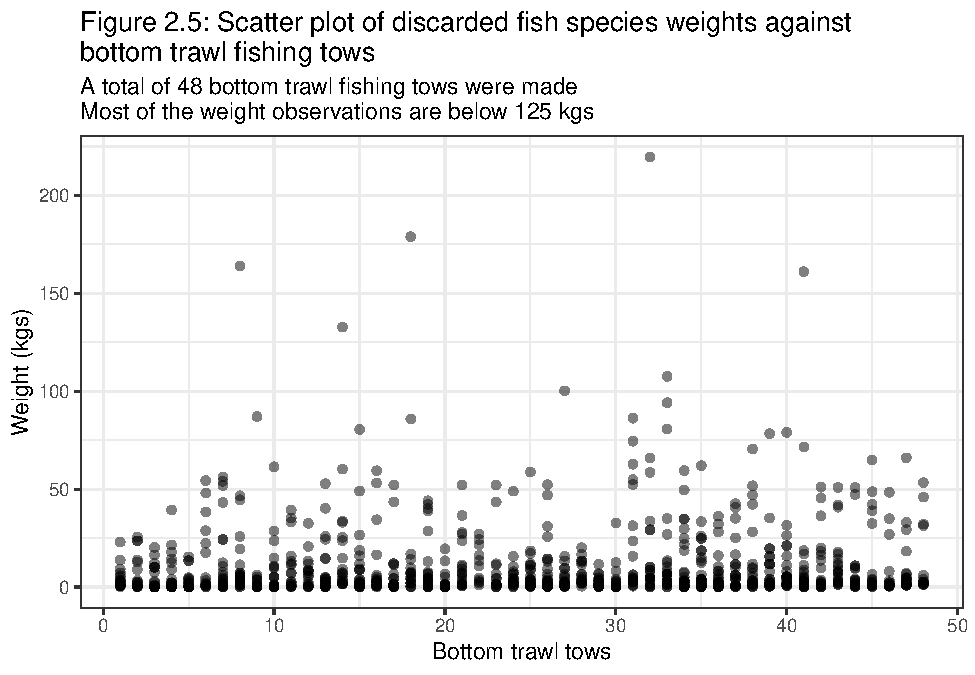
\includegraphics{bookdown-demo_files/figure-latex/unnamed-chunk-17-1} \end{center}

\begin{Shaded}
\begin{Highlighting}[]
\CommentTok{### CODE COMMENTS }\AlertTok{###}
\CommentTok{#[1]. Please see the code comments made at Figure 2.1. }
\end{Highlighting}
\end{Shaded}

Prior to any analysis it is important to inspect the data visually. From the scatter plot (Figure 2.5), we see that for the 48 bottom trawl fishing tows conducted, the weights ranged between 0.0005 kgs to 219.586 kgs. Despite this range most of the points were below 125 kgs. This means that a few data points were \emph{abnormally high}. These points are highlighted below and will subsequently be removed from the analysis, as they were probably mistakes. Again, this decision was guided by my knowledge about the data.

\textbf{Visualizing outliers}

\begin{Shaded}
\begin{Highlighting}[]
\CommentTok{# Subsetting data with outliers}
\NormalTok{Outliers}\FloatTok{.2}\NormalTok{ <-}\StringTok{ }\NormalTok{Discard.data }\OperatorTok\StringTok{ }
\StringTok{  }\KeywordTok{filter}\NormalTok{(TotalWeightKG }\OperatorTok{>}\StringTok{ }\DecValTok{125}\NormalTok{) }

\CommentTok{# Plotting data}
\KeywordTok{ggplot}\NormalTok{(}\DataTypeTok{data =}\NormalTok{ Discard.data) }\OperatorTok{+}
\StringTok{  }\KeywordTok{geom_point}\NormalTok{(}\KeywordTok{aes}\NormalTok{(}\DataTypeTok{x =}\NormalTok{ DragID2,}
    \DataTypeTok{y =}\NormalTok{ TotalWeightKG), }
    \DataTypeTok{alpha =} \FloatTok{0.5}\NormalTok{) }\OperatorTok{+}
\StringTok{  }\KeywordTok{geom_point}\NormalTok{(}\DataTypeTok{data =}\NormalTok{ Outliers}\FloatTok{.2}\NormalTok{,}
    \KeywordTok{aes}\NormalTok{(}\DataTypeTok{x =}\NormalTok{ DragID2,}
      \DataTypeTok{y =}\NormalTok{ TotalWeightKG,}
      \DataTypeTok{color =}\NormalTok{ LatinNames), }
    \DataTypeTok{size =} \DecValTok{3}\NormalTok{) }\OperatorTok{+}
\StringTok{  }\KeywordTok{theme_bw}\NormalTok{() }\OperatorTok{+}
\StringTok{  }\KeywordTok{theme}\NormalTok{(}\DataTypeTok{legend.position =} \StringTok{"bottom"}\NormalTok{,}
    \DataTypeTok{legend.title =} \KeywordTok{element_blank}\NormalTok{()) }\OperatorTok{+}
\StringTok{  }\KeywordTok{guides}\NormalTok{(}\DataTypeTok{color =} \KeywordTok{guide_legend}\NormalTok{(}\DataTypeTok{title =} \StringTok{"Latin Names"}\NormalTok{, }\DataTypeTok{nrow =} \DecValTok{2}\NormalTok{)) }\OperatorTok{+}
\StringTok{  }\KeywordTok{labs}\NormalTok{(}\DataTypeTok{x =} \StringTok{"Bottom trawl fishing tows"}\NormalTok{,}
    \DataTypeTok{y =} \StringTok{"Weight (kgs)"}\NormalTok{,}
    \DataTypeTok{title =} \StringTok{"Figure 2.6: Scatter plot of discarded fish species weights against }\CharTok{\textbackslash{}n}\StringTok{bottom trawl fishing tows"}\NormalTok{,}
    \DataTypeTok{subtitle =} \StringTok{"The oservations above 125 kgs removed - possible outliers"}\NormalTok{)}
\end{Highlighting}
\end{Shaded}

\begin{center}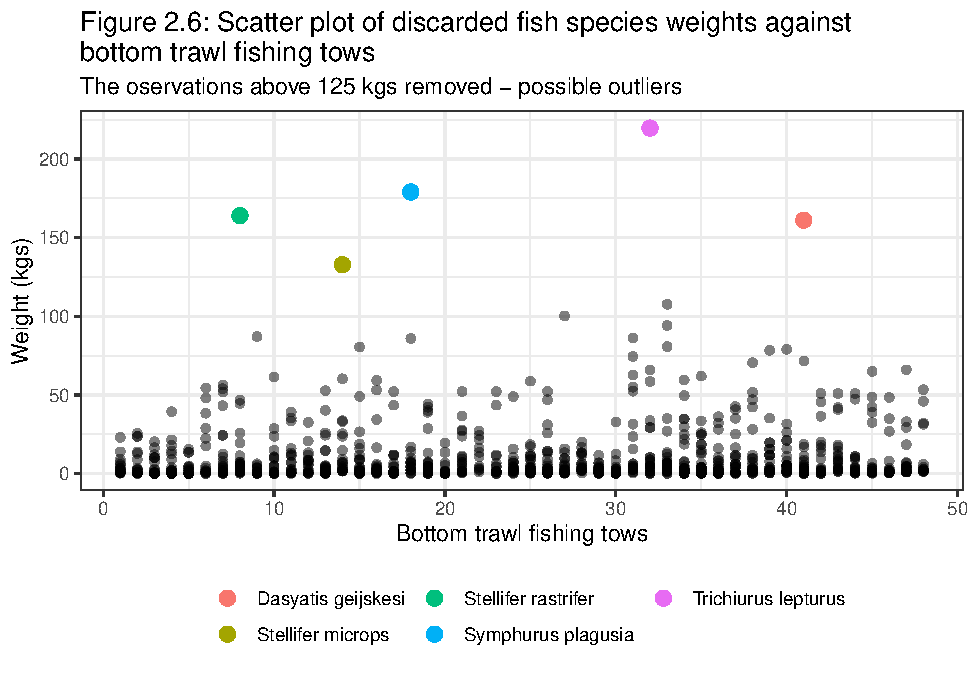
\includegraphics{bookdown-demo_files/figure-latex/unnamed-chunk-18-1} \end{center}

\begin{Shaded}
\begin{Highlighting}[]
\CommentTok{### CODE COMMENTS }\AlertTok{###}
\CommentTok{#[1]. Please see the code comments made at Figure 2.2.  }
\end{Highlighting}
\end{Shaded}

From Figure 2.6 we see that the they were five abnormally high data points. These were for discarded fish species \emph{Dasyatis geijskesi}(peach), \emph{Stellifer rastrifer}(bright green), \emph{Trichiurus lepturus}(purple), \emph{Stellifer microps}(dull green) and \emph{Symphurus plagusia}(blue). As mentioned before these points are strangely high and therefore are perceived to be incorrectly entered and thus will be omitted from the analysis.

\hypertarget{discard-weight-distribution-for-all-fish-species-across-time-of-day-and-fishing-depths.}{%
\subsection{Discard weight distribution for all fish species, across time of day and fishing depths.}\label{discard-weight-distribution-for-all-fish-species-across-time-of-day-and-fishing-depths.}}

\hypertarget{time-of-day}{%
\subsubsection{Time of day}\label{time-of-day}}

\begin{Shaded}
\begin{Highlighting}[]
\CommentTok{# Removing the outliers}
\NormalTok{Discard.data <-}\StringTok{ }\NormalTok{Discard.data }\OperatorTok\StringTok{ }
\StringTok{  }\KeywordTok{filter}\NormalTok{(TotalWeightKG }\OperatorTok{<}\StringTok{ }\DecValTok{125}\NormalTok{)}

\CommentTok{# Summary table - time of day}
\NormalTok{Mean.TP}\FloatTok{.1}\NormalTok{ <-}\StringTok{ }\NormalTok{Discard.data }\OperatorTok\StringTok{ }
\StringTok{  }\KeywordTok{group_by}\NormalTok{(TimePeriods) }\OperatorTok\StringTok{ }
\StringTok{  }\NormalTok{dplyr}\OperatorTok{::}\KeywordTok{summarise}\NormalTok{(}\DataTypeTok{MeanWeight =} \KeywordTok{mean}\NormalTok{(TotalWeightKG), }\DataTypeTok{.groups =} \StringTok{'drop'}\NormalTok{)}

\CommentTok{# Initial plot - time of day}
\KeywordTok{ggplot}\NormalTok{(Discard.data,}
  \KeywordTok{aes}\NormalTok{(TotalWeightKG,}
    \DataTypeTok{color =}\NormalTok{ TimePeriods,}
    \DataTypeTok{fill =}\NormalTok{ TimePeriods)) }\OperatorTok{+}
\StringTok{  }\KeywordTok{geom_density}\NormalTok{(}\DataTypeTok{alpha =} \FloatTok{0.1}\NormalTok{) }\OperatorTok{+}\StringTok{ }
\StringTok{  }\KeywordTok{theme_bw}\NormalTok{() }\OperatorTok{+}
\StringTok{  }\KeywordTok{theme}\NormalTok{(}\DataTypeTok{legend.position =} \StringTok{"bottom"}\NormalTok{) }\OperatorTok{+}
\StringTok{  }\KeywordTok{scale_fill_brewer}\NormalTok{(}\DataTypeTok{palette =} \StringTok{"Set2"}\NormalTok{) }\OperatorTok{+}
\StringTok{  }\KeywordTok{labs}\NormalTok{(}\DataTypeTok{x =} \StringTok{"Weights (kgs)"}\NormalTok{,}
    \DataTypeTok{y =} \StringTok{"Density"}\NormalTok{,}
    \DataTypeTok{title =} \StringTok{"Figure 2.7: Density plot of discarded fish species weight-distribution }\CharTok{\textbackslash{}n}\StringTok{by time of day"}\NormalTok{,}
    \DataTypeTok{subtitle =} \StringTok{"Colours used to represent the different time of day"}\NormalTok{) }\OperatorTok{+}
\StringTok{  }\KeywordTok{geom_vline}\NormalTok{(}\DataTypeTok{data =}\NormalTok{ Mean.TP}\FloatTok{.1}\NormalTok{,}
    \KeywordTok{aes}\NormalTok{(}\DataTypeTok{xintercept =}\NormalTok{ MeanWeight,}
      \DataTypeTok{color =}\NormalTok{ TimePeriods),}
    \DataTypeTok{linetype =} \StringTok{"dotted"}\NormalTok{,}
    \DataTypeTok{size =} \FloatTok{0.5}\NormalTok{) }
\end{Highlighting}
\end{Shaded}

\begin{center}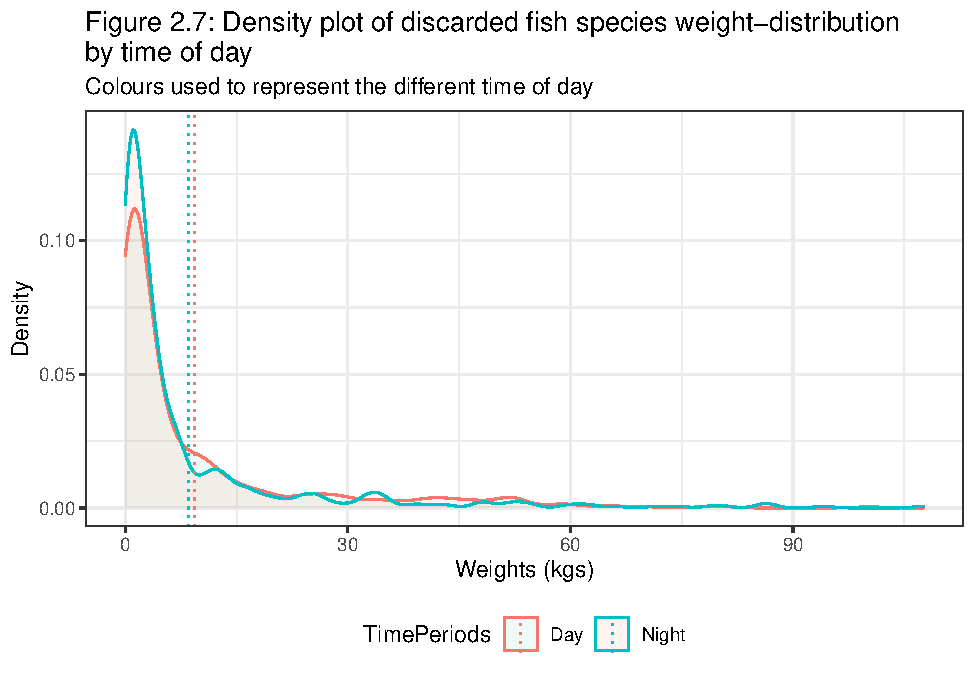
\includegraphics{bookdown-demo_files/figure-latex/unnamed-chunk-19-1} \end{center}

\begin{Shaded}
\begin{Highlighting}[]
\CommentTok{# Summary table with log transformed weights - time of day}
\NormalTok{Mean.TP}\FloatTok{.2}\NormalTok{ <-}\StringTok{ }\NormalTok{Discard.data }\OperatorTok\StringTok{ }
\StringTok{  }\KeywordTok{group_by}\NormalTok{(TimePeriods) }\OperatorTok\StringTok{ }
\StringTok{  }\NormalTok{dplyr}\OperatorTok{::}\KeywordTok{summarise}\NormalTok{(}\DataTypeTok{MeanWeight =} \KeywordTok{mean}\NormalTok{(}\KeywordTok{log10}\NormalTok{(TotalWeightKG)), }\DataTypeTok{.groups =} \StringTok{'drop'}\NormalTok{) }

\CommentTok{# Plotting data on log scale - time of day}
\KeywordTok{ggplot}\NormalTok{(Discard.data,}
  \KeywordTok{aes}\NormalTok{(TotalWeightKG,}
    \DataTypeTok{color =}\NormalTok{ TimePeriods,}
    \DataTypeTok{fill =}\NormalTok{ TimePeriods)) }\OperatorTok{+}
\StringTok{  }\KeywordTok{geom_density}\NormalTok{(}\DataTypeTok{alpha =} \FloatTok{0.1}\NormalTok{) }\OperatorTok{+}\StringTok{ }
\StringTok{  }\KeywordTok{theme_bw}\NormalTok{() }\OperatorTok{+}
\StringTok{  }\KeywordTok{theme}\NormalTok{(}\DataTypeTok{legend.position =} \StringTok{"bottom"}\NormalTok{) }\OperatorTok{+}
\StringTok{  }\KeywordTok{scale_fill_brewer}\NormalTok{(}\DataTypeTok{palette =} \StringTok{"Set2"}\NormalTok{) }\OperatorTok{+}
\StringTok{  }\KeywordTok{labs}\NormalTok{(}\DataTypeTok{x =} \StringTok{"Weights (Log Scale)"}\NormalTok{,}
    \DataTypeTok{y =} \StringTok{"Density"}\NormalTok{,}
    \DataTypeTok{title =} \StringTok{"Figure 2.8: Density plot of discarded fish species weight-distribution }\CharTok{\textbackslash{}n}\StringTok{by time of day"}\NormalTok{,}
    \DataTypeTok{subtitle =} \StringTok{"Colours used to represent the different time of day"}\NormalTok{) }\OperatorTok{+}
\StringTok{  }\KeywordTok{scale_x_continuous}\NormalTok{(}\DataTypeTok{trans =} \StringTok{"log10"}\NormalTok{) }\OperatorTok{+}
\StringTok{  }\KeywordTok{geom_vline}\NormalTok{(}\DataTypeTok{data =}\NormalTok{ Mean.TP}\FloatTok{.2}\NormalTok{,}
    \KeywordTok{aes}\NormalTok{(}\DataTypeTok{xintercept =}\NormalTok{ MeanWeight,}
      \DataTypeTok{color =}\NormalTok{ TimePeriods),}
    \DataTypeTok{linetype =} \StringTok{"dotted"}\NormalTok{,}
    \DataTypeTok{size =} \FloatTok{0.5}\NormalTok{) }
\end{Highlighting}
\end{Shaded}

\begin{center}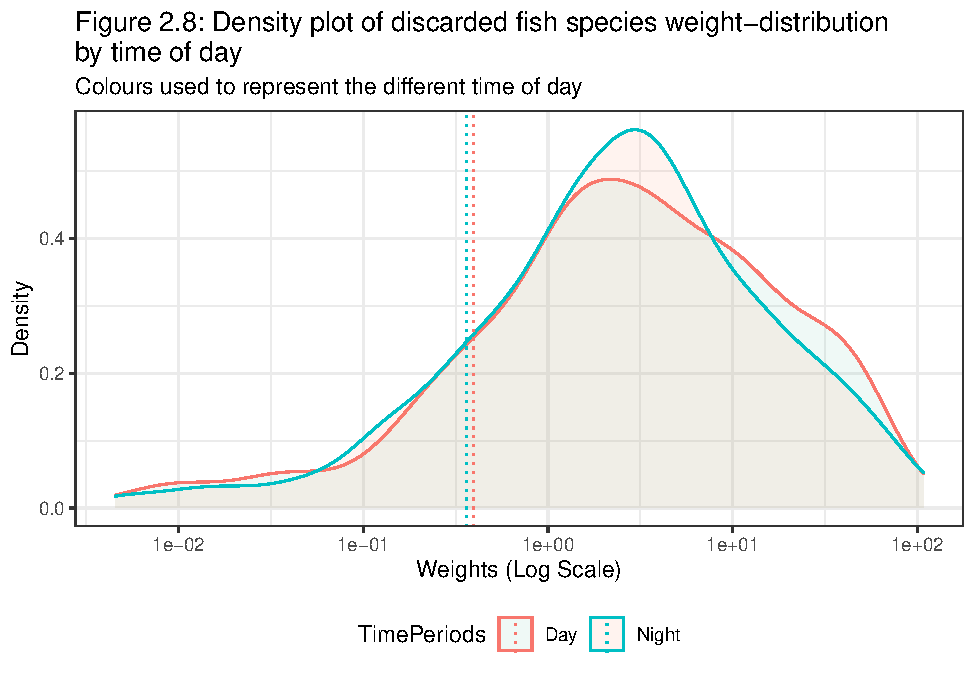
\includegraphics{bookdown-demo_files/figure-latex/unnamed-chunk-19-2} \end{center}

\begin{Shaded}
\begin{Highlighting}[]
\CommentTok{### CODE COMMENTS }\AlertTok{###}
\CommentTok{#[1]. The code comments made in the earlier Tables and Figures mostly apply here too except that: }
\CommentTok{#[2]. log10() is used to transform the weight data to a log scale in the "Mean.TP.2" object. }
\CommentTok{#     This was done to create the vertical line (using geom_vline()) of the group }
\CommentTok{#     means in Figure 2.6. }
\CommentTok{#[3]. fill() is passed to mapping = aes() to group and color the data by time of day. }
\CommentTok{#[4]. scale_x_continuous() is used with the "trans" argument to log transform the data to the base 10. }
\CommentTok{#[5]. geom_vline() is used to add vertical lines showing the "mean weights" by time of day on the }
\CommentTok{#     density plots. These are highlighted by the arguments color, linetype and size.  }
\CommentTok{#[6]. Otherwise, please see code comments made at "Table.2.1", "Figure 2.3" and the other}
\CommentTok{#     Tables and Figures in this submission. }
\end{Highlighting}
\end{Shaded}

From the density plot shown in Figure 2.7 we can see that the data is skewed to the right. The reason for this is that the data is recorded by fish species observations and usually the very small fish species are discarded. The weights for all fish species ranged from 0.005 kgs to 100 kgs in the day and 0.005 kgs to 108 kgs in the night. The mean weight for all fish species was higher in the day (9.37 kgs) in comparison to the night (8.53 kgs). To better see these distributions the data was log transformed and presented in Figure 2.8. From this plot we can see the weight distribution clearer, hence log transforming the data worked reasonably fine.

\hypertarget{fishing-depths}{%
\subsubsection{Fishing depths}\label{fishing-depths}}

\begin{Shaded}
\begin{Highlighting}[]
\CommentTok{# Summary table - fishing depths}
\NormalTok{Mean.FD}\FloatTok{.1}\NormalTok{ <-}\StringTok{ }\NormalTok{Discard.data }\OperatorTok\StringTok{ }
\StringTok{  }\KeywordTok{group_by}\NormalTok{(FishingDepth2) }\OperatorTok\StringTok{ }
\StringTok{  }\NormalTok{dplyr}\OperatorTok{::}\KeywordTok{summarise}\NormalTok{(}\DataTypeTok{MeanWeight =} \KeywordTok{mean}\NormalTok{(TotalWeightKG),}
    \DataTypeTok{.groups =} \StringTok{'drop'}\NormalTok{)}

\CommentTok{# Initial plot - fishing depths}
\KeywordTok{ggplot}\NormalTok{(Discard.data,}
  \KeywordTok{aes}\NormalTok{(TotalWeightKG,}
    \DataTypeTok{color =}\NormalTok{ FishingDepth2,}
    \DataTypeTok{fill =}\NormalTok{ FishingDepth2)) }\OperatorTok{+}
\StringTok{  }\KeywordTok{geom_density}\NormalTok{(}\DataTypeTok{alpha =} \FloatTok{0.1}\NormalTok{) }\OperatorTok{+}\StringTok{ }
\StringTok{  }\KeywordTok{theme_bw}\NormalTok{() }\OperatorTok{+}
\StringTok{  }\KeywordTok{theme}\NormalTok{(}\DataTypeTok{axis.text =} \KeywordTok{element_text}\NormalTok{(}\DataTypeTok{size =} \DecValTok{10}\NormalTok{),}
    \DataTypeTok{axis.title =} \KeywordTok{element_text}\NormalTok{(}\DataTypeTok{size =} \DecValTok{10}\NormalTok{),}
    \DataTypeTok{legend.position =} \StringTok{"bottom"}\NormalTok{) }\OperatorTok{+}
\StringTok{  }\KeywordTok{labs}\NormalTok{(}\DataTypeTok{x =} \StringTok{"Weights (Log Scale)"}\NormalTok{,}
    \DataTypeTok{y =} \StringTok{"Density"}\NormalTok{,}
    \DataTypeTok{title =} \StringTok{"Figure 2.9: Density plot of discarded fish species weight-distribution }\CharTok{\textbackslash{}n}\StringTok{by fishing depths"}\NormalTok{,}
    \DataTypeTok{subtitle =} \StringTok{"Colours used to represent the different fishing depths"}\NormalTok{) }\OperatorTok{+}
\StringTok{  }\KeywordTok{geom_vline}\NormalTok{(}\DataTypeTok{data =}\NormalTok{ Mean.FD}\FloatTok{.1}\NormalTok{,}
    \KeywordTok{aes}\NormalTok{(}\DataTypeTok{xintercept =}\NormalTok{ MeanWeight,}
      \DataTypeTok{color =}\NormalTok{ FishingDepth2),}
    \DataTypeTok{linetype =} \StringTok{"dotted"}\NormalTok{,}
    \DataTypeTok{size =} \FloatTok{0.5}\NormalTok{)}
\end{Highlighting}
\end{Shaded}

\begin{center}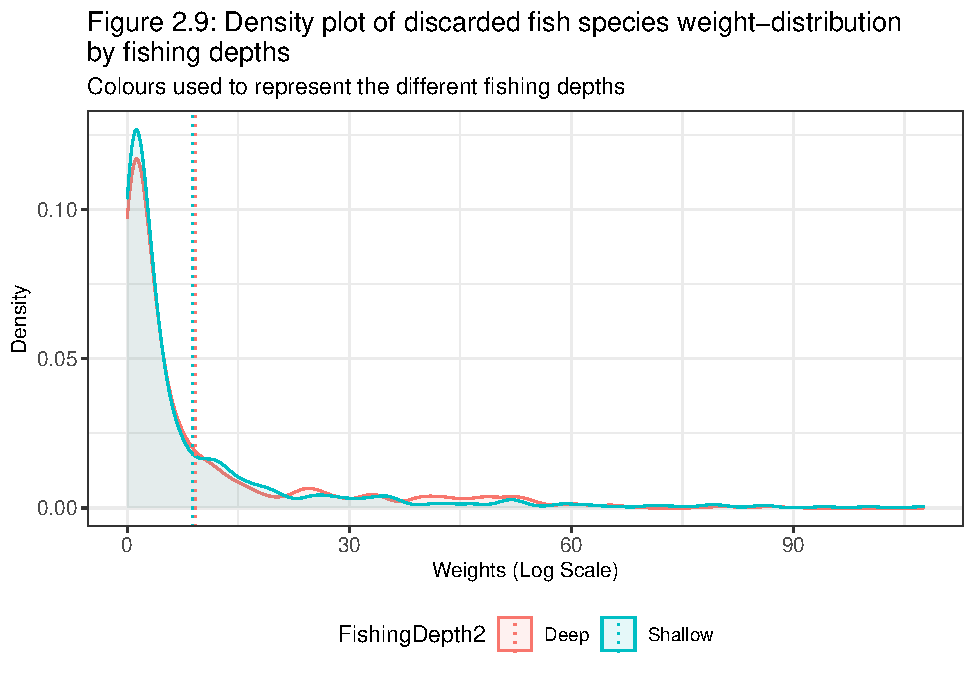
\includegraphics{bookdown-demo_files/figure-latex/unnamed-chunk-20-1} \end{center}

\begin{Shaded}
\begin{Highlighting}[]
\CommentTok{# Summary table with log transformed weights - fishing depths}
\NormalTok{Mean.FD}\FloatTok{.2}\NormalTok{ <-}\StringTok{ }\NormalTok{Discard.data }\OperatorTok\StringTok{ }
\StringTok{  }\KeywordTok{group_by}\NormalTok{(FishingDepth2) }\OperatorTok\StringTok{ }
\StringTok{  }\NormalTok{dplyr}\OperatorTok{::}\KeywordTok{summarise}\NormalTok{(}\DataTypeTok{MeanWeight =} \KeywordTok{mean}\NormalTok{(}\KeywordTok{log10}\NormalTok{(TotalWeightKG)), }\DataTypeTok{.groups =} \StringTok{'drop'}\NormalTok{)}

\CommentTok{# Table with log transformed weights - fishing depths}
\KeywordTok{ggplot}\NormalTok{(Discard.data,}
  \KeywordTok{aes}\NormalTok{(TotalWeightKG,}
    \DataTypeTok{color =}\NormalTok{ FishingDepth2,}
    \DataTypeTok{fill =}\NormalTok{ FishingDepth2)) }\OperatorTok{+}
\StringTok{  }\KeywordTok{geom_density}\NormalTok{(}\DataTypeTok{alpha =} \FloatTok{0.1}\NormalTok{) }\OperatorTok{+}\StringTok{ }
\StringTok{  }\KeywordTok{theme_bw}\NormalTok{() }\OperatorTok{+}
\StringTok{  }\KeywordTok{theme}\NormalTok{(}\DataTypeTok{axis.text =} \KeywordTok{element_text}\NormalTok{(}\DataTypeTok{size =} \DecValTok{10}\NormalTok{),}
    \DataTypeTok{axis.title =} \KeywordTok{element_text}\NormalTok{(}\DataTypeTok{size =} \DecValTok{10}\NormalTok{),}
    \DataTypeTok{legend.position =} \StringTok{"bottom"}\NormalTok{) }\OperatorTok{+}
\StringTok{  }\KeywordTok{labs}\NormalTok{(}\DataTypeTok{x =} \StringTok{"Weights (Log Scale)"}\NormalTok{,}
    \DataTypeTok{y =} \StringTok{"Density"}\NormalTok{,}
    \DataTypeTok{title =} \StringTok{"Figure 2.10: Density plot of discarded fish species weight-distribution }\CharTok{\textbackslash{}n}\StringTok{by fishing depths"}\NormalTok{,}
    \DataTypeTok{subtitle =} \StringTok{"Colours used to represent the different fishing depths"}\NormalTok{) }\OperatorTok{+}
\StringTok{  }\KeywordTok{scale_x_continuous}\NormalTok{(}\DataTypeTok{trans =} \StringTok{"log10"}\NormalTok{) }\OperatorTok{+}
\StringTok{  }\KeywordTok{geom_vline}\NormalTok{(}\DataTypeTok{data =}\NormalTok{ Mean.FD}\FloatTok{.2}\NormalTok{,}
    \KeywordTok{aes}\NormalTok{(}\DataTypeTok{xintercept =}\NormalTok{ MeanWeight,}
      \DataTypeTok{color =}\NormalTok{ FishingDepth2),}
    \DataTypeTok{linetype =} \StringTok{"dotted"}\NormalTok{,}
    \DataTypeTok{size =} \FloatTok{0.5}\NormalTok{)}
\end{Highlighting}
\end{Shaded}

\begin{center}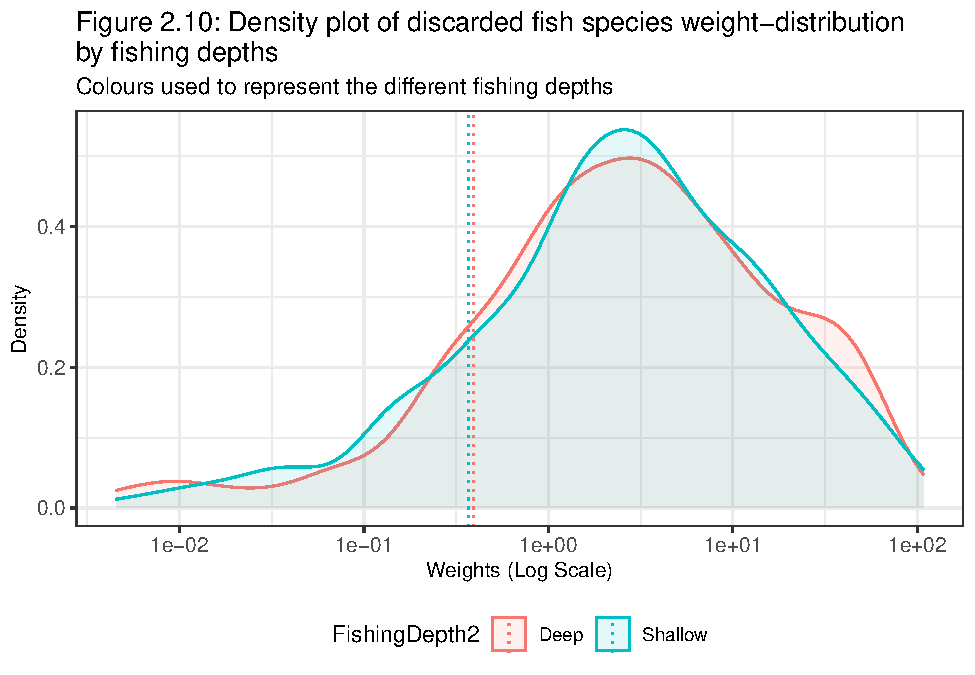
\includegraphics{bookdown-demo_files/figure-latex/unnamed-chunk-20-2} \end{center}

\begin{Shaded}
\begin{Highlighting}[]
\CommentTok{### CODE COMMENTS }\AlertTok{###}
\CommentTok{#[1]. To see a description of what the functions in these code are doing please refer to }
\CommentTok{#     the code comments made at Figures 2.7 and 2.8 and in the Mean.TP.1 and Mean.TP.2 tables.}
\CommentTok{#     The only exception is that "TimePeriods" i.e. time of day, is replaced with }
\CommentTok{#     "FishingDepth2" i.e. fishing depths. }
\end{Highlighting}
\end{Shaded}

From the density plot shown in Figure 2.9 we can see that the data is again skewed to the right. The reason for this is the same i.e.~that the data is recorded by fish species observations and usually the very small fish species are discarded. The weights for all fish species ranged from 0.005 kgs to 87 kgs in the deep and 0.005 kgs to 108 kgs in the shallow. The mean weight for all fish species was higher in the deep (9.16 kgs) in comparison to the shallow (8.80 kgs). To better see these distributions the data was log transformed and presented in Figure 2.10. From this plot we can see the weight distribution clearer, hence log transforming the data worked reasonably fine.

\hypertarget{analysis-of-the-mean-discarded-catch-across-time-periods-and-fishing-depths-using-the-welch-two-sample-t-test.}{%
\subsection{\texorpdfstring{Analysis of the mean discarded catch across time-Periods and fishing depths using the \textbf{Welch Two Sample t-test}.}{Analysis of the mean discarded catch across time-Periods and fishing depths using the Welch Two Sample t-test.}}\label{analysis-of-the-mean-discarded-catch-across-time-periods-and-fishing-depths-using-the-welch-two-sample-t-test.}}

\textbf{Test assumptions}

This test assumes that the the weight observations across time of day (day/night) and fishing depths (deep/shallow) are normally distributed. Fortunately as well, this method is not at all sensitive to deviations from this assumption. Therefore, if the distributions of day/night or deep/shallow are the same e.g.~if both distributions are skewed to the right. This example is the case with this data as seen earlier. This means that the analysis will be performed on the actual weights variable and no transformation is needed. \textbf{This assumption was tested in this project and the results indeed were almost identical}

\textbf{How the Welch Two Sample t-test works}

The test statistic, \(t_s\), is computed using a method that has the difference between the means in the numerator. This therefore makes the \(t_s\) larger as the means move away from each other. The standard error of the difference in the means in this case is denominator. This value decreases as the sample variances decreases or if the size of sample increase. Hence the \(t_s\) gets larger as the means move further apart, the variances get smaller, or if the size of the sample increase. The probability of getting the observed \(t_s\) value under the \textbf{null hypothesis} is computed using the t-distribution.

\textbf{Conducting the t-tests}

\hypertarget{time-of-day-1}{%
\subsubsection{Time of day}\label{time-of-day-1}}

\begin{Shaded}
\begin{Highlighting}[]
\CommentTok{# Welch t.test - time of day}
\NormalTok{Weight.ttest.TP <-}\StringTok{ }\KeywordTok{t.test}\NormalTok{(TotalWeightKG }\OperatorTok{~}\StringTok{ }\NormalTok{TimePeriods,}
  \DataTypeTok{data =}\NormalTok{ Discard.data)}

\NormalTok{Weight.ttest.TP}
\end{Highlighting}
\end{Shaded}

\begin{verbatim}
  
    Welch Two Sample t-test
  
  data:  TotalWeightKG by TimePeriods
  t = 0.89664, df = 1056.3, p-value = 0.3701
  alternative hypothesis: true difference in means is not equal to 0
  95 percent confidence interval:
   -0.9953903  2.6705615
  sample estimates:
    mean in group Day mean in group Night 
             9.370018            8.532433
\end{verbatim}

\begin{Shaded}
\begin{Highlighting}[]
\CommentTok{### CODE COMMENTS }\AlertTok{###}
\CommentTok{#[1]. The "DiscardData" is passed to t.test(). }
\CommentTok{#[2]. t.test() is used to analyze the "TotalWeightKG" variable against time-periods. }
\end{Highlighting}
\end{Shaded}

The p-value associated with the test is \(0.37\), so we cannot reject the null hypothesis (\(H_0\)) of no difference between the (true) means of the two groups (i.e.~time of day; day and night) since the p-value is greater than the usual significance level \(alpha = 0.05\). Therefore we conclude based on this data, that there is not enough evidence of a difference between the (true) means of the two groups at the usual significance level of \(alpha = 0.05\).

\hypertarget{fishing-depths-1}{%
\subsubsection{Fishing depths}\label{fishing-depths-1}}

\begin{Shaded}
\begin{Highlighting}[]
\CommentTok{# Welch t.test - fishing depths}
\NormalTok{Weight.ttest.FD <-}\StringTok{ }\KeywordTok{t.test}\NormalTok{(TotalWeightKG }\OperatorTok{~}\StringTok{ }\NormalTok{FishingDepth2,}
  \DataTypeTok{data =}\NormalTok{ Discard.data)}

\NormalTok{Weight.ttest.FD}
\end{Highlighting}
\end{Shaded}

\begin{verbatim}
  
    Welch Two Sample t-test
  
  data:  TotalWeightKG by FishingDepth2
  t = 0.39181, df = 1050.8, p-value = 0.6953
  alternative hypothesis: true difference in means is not equal to 0
  95 percent confidence interval:
   -1.461899  2.191380
  sample estimates:
     mean in group Deep mean in group Shallow 
               9.163561              8.798821
\end{verbatim}

\begin{Shaded}
\begin{Highlighting}[]
\CommentTok{### CODE COMMENTS }\AlertTok{###}
\CommentTok{#[1]. To see a description of what the functions in this code are doing please refer to}
\CommentTok{#     the code comments at Weight.ttest.TP. The only exception is "FishingDepth2" }
\CommentTok{#     have replaced "TimePeriods". }
\end{Highlighting}
\end{Shaded}

The p-value associated with the test is \(0.70\), so we cannot reject the null hypothesis (\(H_0\)) of no difference between the (true) means of the two groups (i.e.~fishing depths; deep and shallow) since the p-value is greater than the usual significance level \(alpha = 0.05\). Therefore we conclude dased on this data, that there is not enough evidence of a difference between the (true) means of the two groups at the usual significance level of \(alpha = 0.05\).

\hypertarget{analysis-summary}{%
\subsection{Analysis summary}\label{analysis-summary}}

In summary, from the analysis of the discarded species (ALL) from the data, we found that there is not enough evidence to reject the null hypothesis (\(H_0\)) which is that \emph{the means are equal across time of day and fishing depths}. This was proven by the high p-values (\(> 0.05\)) obtained from the Welch Two Sample t-tests conducted on the discard species data across time of day and fishing depths.

\hypertarget{closing-remarks}{%
\section{Closing remarks}\label{closing-remarks}}

This submission focused on the \textbf{weight analysis} of discarded fish species. In the next submission, the focus will be on the \textbf{length analysis} of discarded fish species. To achieve this a separate dataset will be \textbf{joined} to the data used in this submission. This will be required to answer \textbf{Research Questions 5 \& 6}. For more details please see \textbf{Submission One} - section 1.2.

\hypertarget{appendix}{%
\chapter{Appendix}\label{appendix}}

\hypertarget{bottom-trawl-fishing-vessel}{%
\section{Bottom trawl fishing vessel}\label{bottom-trawl-fishing-vessel}}

\begin{figure}
\centering
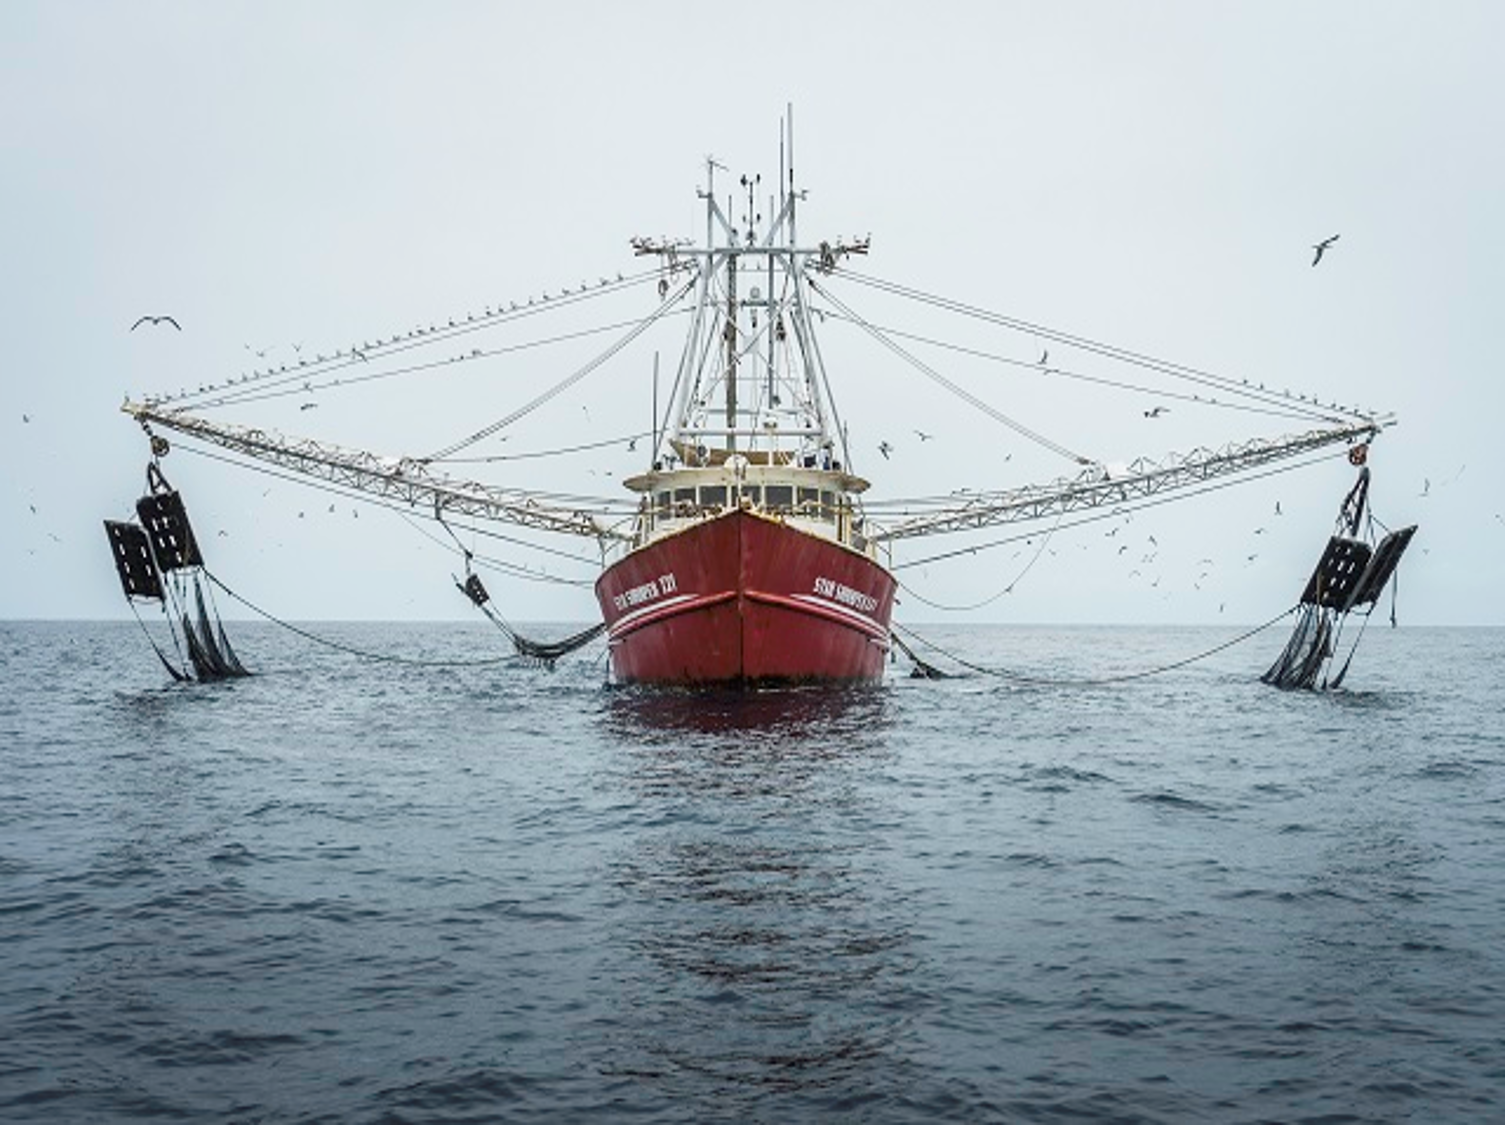
\includegraphics[width=0.6\textwidth,height=\textheight]{C:/Users/UNUFTP/Documents/mas102m/BottomTrawl.png}
\caption{A typical bottom trawl fishing vessel used in Guyana (The Maritime Executive, 2020)}
\end{figure}

\hypertarget{discarded-fish-species}{%
\section{Discarded fish species}\label{discarded-fish-species}}

\begin{figure}
\centering
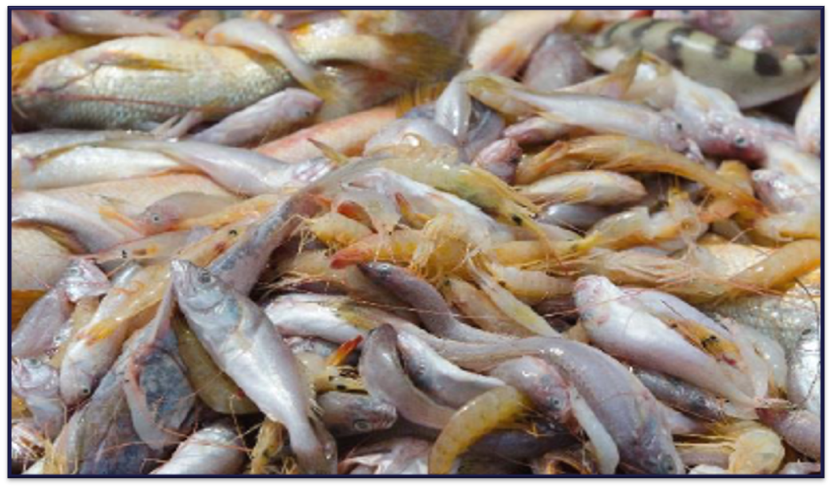
\includegraphics[width=0.6\textwidth,height=\textheight]{C:/Users/UNUFTP/Documents/mas102m/Discards.png}
\caption{An example of fish species discarded (Richardson, 2018)}
\end{figure}

\hypertarget{atlantic-seabob-shrimp}{%
\section{Atlantic seabob shrimp}\label{atlantic-seabob-shrimp}}

\begin{figure}
\centering
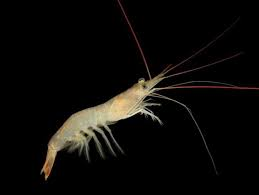
\includegraphics[width=0.6\textwidth,height=\textheight]{C:/Users/UNUFTP/Documents/mas102m/Seabob.jpg}
\caption{A typical photo of an Atlantic seabob shrimp caught offshore Guyana(Torrez, 2015)}
\end{figure}

  \bibliography{book.bib,packages.bib}

\end{document}
